% !TeX spellcheck = fr_FR
\documentclass[12pt, openany]{report}
\usepackage[utf8]{inputenc}
\usepackage[T1]{fontenc}
\usepackage[a4paper,left=2cm,right=2cm,top=2cm,bottom=2cm]{geometry}
\usepackage[frenchb]{babel}
\usepackage{libertine}
\usepackage[pdftex]{graphicx}
\usepackage{amssymb}
\usepackage{listings}
\usepackage{color}
\usepackage[dvipsnames]{xcolor}


\usepackage[colorlinks=true,linkcolor=red]{hyperref}
\usepackage[nottoc, notlof, notlot]{tocbibind}

\usepackage{cite}

%Defines a new environment for java code (use \begin{java})
\lstnewenvironment{java}[1][]%
{
	\noindent
	\minipage{\linewidth} 
	\vspace{0.5\baselineskip}
	\lstset{language=Java,                  % the language of the code
		basicstyle=\footnotesize,       % the size of the fonts that are used for the code
		numbers=left,                   % where to put the line-numbers
		numberstyle=\tiny\color{Brown},  % the style that is used for the line-numbers
		stepnumber=1,                   % the step between two line-numbers. If it's 1, each line 
		% will be numbered
		numbersep=5pt,                  % how far the line-numbers are from the code
		backgroundcolor=\color{white},  % choose the background color. You must add \usepackage{color}
		showspaces=false,               % show spaces adding particular underscores
		showstringspaces=false,         % underline spaces within strings
		showtabs=false,                 % show tabs within strings adding particular underscores
		frame=single,                   % adds a frame around the code
		rulecolor=\color{black},        % if not set, the frame-color may be changed on line-breaks within not-black text (e.g. commens (green here))
		tabsize=4,                      % sets default tabsize to 2 spaces
		captionpos=b,                   % sets the caption-position to bottom
		breaklines=true,                % sets automatic line breaking
		breakatwhitespace=false,        % sets if automatic breaks should only happen at whitespace
		title=\lstname,                 % show the filename of files included with \lstinputlisting;
		% also try caption instead of title
		keywordstyle=\color{blue},          % keyword style
		commentstyle=\color{dkgreen},       % comment style
		stringstyle=\color{mauve},         % string literal style
		escapeinside={\%*}{*)},            % if you want to add a comment within your code
		morekeywords={*,...}               % if you want to add more keywords to the set
		}}
{\endminipage}

\setlength{\parindent}{1cm}
\setlength{\parskip}{1ex plus 0.5ex minus 0.2ex}
\newcommand{\hsp}{\hspace{20pt}}
\newcommand{\HRule}{\rule{\linewidth}{0.5mm}}
\begin{document}

\begin{titlepage}
  \begin{sffamily}
  \begin{center}

    
\includegraphics[scale=0.2]{Images/UMONS+txt.png}   ~\\[1.5cm]
    


    \HRule \\[0.4cm]
    { \huge \bfseries Projet de Software Evolution - JPacman\\[0.4cm] }
    \HRule \\[2cm]
    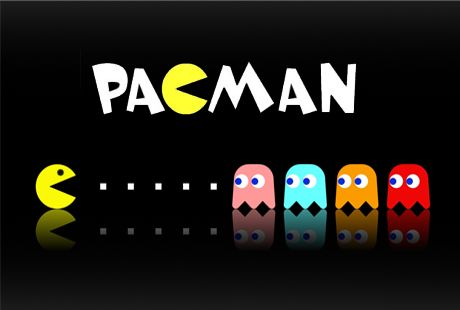
\includegraphics[scale=0.5]{Images/Pac-Man.jpg}~\\[1.5cm] 

    
    

    \begin{minipage}{0.4\textwidth}
      \begin{flushleft} \large
        \emph{Réalisateurs :\\} Damien \textsc{Legay}\\ Adrien \textsc{Coppens}\\ Nicolas \textsc{Leemans}\\
        
      \end{flushleft}
    \end{minipage}
    \begin{minipage}{0.4\textwidth}
      \begin{flushright} \large
        \emph{Enseignant :} M. Tom  \textsc{Mens}\\
        \emph{Date de remise : } 9 mai 2016\\
        \emph{Année d'étude : } Master 1
      \end{flushright}
    \end{minipage}

    \vfill

    {\large Année académique 2015 - 2016}
	
  \end{center}
  \end{sffamily}
\end{titlepage}


	\setcounter{secnumdepth}{3}
	\setcounter{tocdepth}{3}

\newpage

	\renewcommand{\thesection}{\arabic{section}}
	\tableofcontents
	\newpage

	

\section{Introduction}
%todo: uniformiser : \textit{Class#Method} ? (==javadoc) + préciser convention au début du rapport
Ce projet, effectué dans le cadre du cours de "Software Evolution" dispensé par le Professeur Tom Mens durant l'année académique 2015-2016, a pour but de mettre en pratique les concepts d'évolution logicielle vus au cours théorique. Il consiste à analyser et à étendre un projet en effectuant un contrôle de la qualité au travers de différentes métriques, le \textit{"refactoring"} du code source, ainsi que l'implémentation de nouvelles fonctionnalités. Le projet concerné s'appelle JPacman\footnote{https://github.com/SERG-Delft/jpacman-framework}. Il s'agit d'une implémentation très basique du jeu Pacman en Java, créé par l'équipe  du Professeur Arie van Deursen, à Delft University of Technology (Pays-Bas).
 JPacman contient plusieurs simplifications par rapport au jeu Pac-Man original. Le jeu consiste à déplacer Pac-Man, un personnage qui, vu de profil, ressemble à un diagramme circulaire à l’intérieur d’un labyrinthe, afin de lui faire manger toutes les pac-gommes qui s’y trouvent en évitant d’être touché par des fantômes.
 
Ce rapport s'organise en plusieurs parties. La première section présente les différentes extensions qui ont été réalisées à partir de la version originale de JPacman. La seconde section met en avant les principaux problèmes de conflits rencontrés lors de l'intégration des extensions individuelles et leurs résolutions. Ensuite, la troisième section traite des \textit{refactorings} qui ont été réalisés avant l'analyse de la qualité. La prochaine section présente une comparaison entre la qualité du code source finale avec la qualité du code source original. Ensuite, la section suivante définit une analyse de l'évolution du logiciel en terme de nombres de lignes de code. Pour finir, un complément d'information concernant l'utilisation du logiciel est fourni dans la dernière partie de ce rapport. 


\section{Extension du logiciel}\label{extensions}

La première partie de ce projet consistait à étendre la version initiale de JPacman en ajoutant de nouvelles fonctionnalités et en suivant un processus de développement dirigé par les tests. De nouveaux tests unitaires ont donc été ajoutés pour chaque fonctionnalité afin de vérifier que le comportement initial du logiciel n’a pas été altéré. 

Chaque membre du groupe a donc implémenté une des fonctionnalités suivantes :
\begin{itemize}
\item L'implémentation d'un score (réalisée par Damien Legay)
\item L'implémentation d'une série de labyrinthes (réalisée par Adrien Coppens)
\item L'implémentation d'une intelligence artificielle pour pacman (réalisée par Nicolas Leemans)
\end{itemize}


\subsection{Fonctionnalité "Score"}\label{score}
Cette fonctionnalité requiert l'implémentation de deux sous-fonctionnalités:

La première fonctionnalité (Hall of Fame) consiste à maintenir une liste de hauts scores. Si un joueur dépasse l'un des dix meilleurs scores, son nom doit être inséré dans le Hall of Fame.
Ceci peut être réalisé de deux manières différentes: si le joueur est identifié, son nom de joueur sera automatiquement entré, si ce n'est pas le cas, il lui sera demandé de fournir un nom à la fin de la partie.
Le score du joueur est affecté par le nombre de gommes, fantômes et fruits consommés par Pacman, ainsi que par les hauts faits réalisés (voir ci-bas).

Lorsque la partie est terminée, le Hall of Fame est affiché et le joueur a l'option de le réinitialiser à ses valeurs par défaut. Pour éviter que celle-ci ne se fasse par mégarde, une confirmation est demandée.

La deuxième fonctionnalité (Achievements) implique d'implémenter un système de gestion de hauts faits. 
Pour ce faire, un système de profils doit être mis en place, permettant au joueur la possibilité de s'identifier et ainsi réaliser des hauts faits qui sont mémorisés.
Ces hauts faits peuvent être accomplis sur plusieurs parties indépendantes.
Le joueur doit avoir la possibilité de visualiser les hauts faits qu'il a accompli avant de commencer à jouer, à la suite de quoi le jeu proposera de nouveaux haut faits à réaliser, au maximum de trois.
Lorsque le joueur obtient un haut fait, il reçoit un bonus de score.

Pour réaliser ces fonctionnalités, il a d'abord convenu d'associer à chaque élément pouvant être consommé par Pacman une valeur numérique à ajouter au score, même pour les éléments que Pacman ne peut pas manger à ce stade puisque dépendants de fonctionnalités non implémentées (fruits, supergomme pour manger les fantômes).
Ces valeurs sont localisées dans les classes \mbox{\textit{LevelFactory}} (gommes et fruits) et \mbox{\textit{Ghost}} (fantômes).

Ensuite, un système de Hall of Fame a été mis en place à l'aide de la classe \mbox{\textit{HallOfFame}} qui offre les services suivants:

\begin{enumerate}
\item La méthode \mbox{\textit{HallOfFame\#handleHoF()}} se charge de mettre à jour le Hall of Fame si nécessaire, c'est à dire si le score du joueur excède l'un des scores sauvegardés dans le fichier \mbox{\textit{resources\\HoF.txt}}, et de l'afficher qu'il ait été mis à jour ou non.
\item La méthode \mbox{\textit{HallOfFame\#resetHoF()}}, quant à elle, a pour rôle de réinitialiser le Hall of Fame aux valeurs par défaut telles que définies dans le fichier \mbox{\textit{resources\\DefaultHoF.txt}}.
\end{enumerate}

\begin{figure}[h]
	\centering
	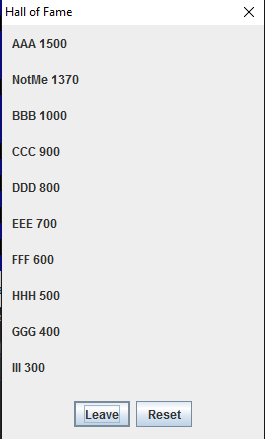
\includegraphics[width=6cm]{Images/HoF.png}
	\caption{\label{hof} Le Hall of Fame après que le joueur "NotMe" a terminé une partie}
\end{figure}


Enfin, un système de gestion des hauts faits a été réalisé. Pour cela, il a été nécessaire de mettre en œuvre un système d'authentification du joueur.
Ce système repose sur les éléments que voici:

\begin{enumerate}
\item Le fichier \mbox{\textit{resources\\login.txt}}, dans lequel sont stockés les identifiants et mots de passes (non en clair) des joueurs ;
\item Le répertoire \mbox{\textit{resources\\profiles\\}}, qui contient les profils des joueurs ayant créé un compte.
Le format des fichiers .prf contenus dans ce répertoire est tel que suit: 
\begin{itemize}
\item La première ligne contient des informations diverses : score maximal atteint par le joueur, nombre fois qu'il a été tué par tel fantôme, niveau maximum que le joueur a complété,...
\item Les lignes suivantes contiennent le nom d'un haut fait accompli par le joueur.
\end{itemize}
\item La méthode \mbox{\textit{IdentifiedPlayer\#createNewPlayer()}}, qui permet à un joueur de créér un nouveau profil joueur, et, si besoin est, le répertoire ci-dessus ;
\item La méthode \mbox{\textit{IdentifiedPlayer\#authenticate()}}, qui vérifie que l'identifiant et le mot de passe entrés par le joueur correspondent bien à des données situées dans \mbox{\textit{resources\\login.txt}} et, si le joueur le désire, affiche les hauts faits qu'il a déjà obtenus ;
\item La méthode \mbox{\textit{IdentifiedPlayer\#addAchievement()}}, servant à ajouter un haut fait que le joueur a obtenu dans son fichier profil, si celui-ci ne s' y trouve déjà ;
\item La méthode \mbox{\textit{IdentifiedPlayer\#saveScore()}}, qui met à jour le score maximal du joueur et lui accorde les hauts faits liés à celui-ci ;
\item La méthode \mbox{\textit{IdentifiedPlayer\#killedBy()}}, mettant à jour les informations liées au fait de s'être fait tuer par un fantôme et affectant les hauts faits correspondants ;
\item La méthode \mbox{\textit{IdentifiedPlayer\#levelCompleted()}} en fait de même pour le niveau maximal atteint ;
\item La méthode \mbox{\textit{IdentifiedPlayer\#displayProfileStats()}}, qui affiche les informations concernant le joueur, s'il est identifié, et lui propose d'en accomplir d'autres, s'il n'a pas accompli tous les hauts faits disponibles ;
\item La classe utilitaire \mbox{\textit{FileChecker}} qui effectue certaines opérations de vérification sur les fichiers susnommés ;
\item L'énumération \mbox{\textit{Achievement}} dans laquelle sont stockés les hauts faits, le score qu'ils accordent lorsqu'ils sont accomplis, une description définissant comment les obtenir et le haut fait à recommencer après leur obtention.
\end{enumerate}


\subsection{Fonctionnalité "Série de labyrinthes"}\label{labyrinthe}
Les ajouts à effectuer pour cette extension sont :
\begin{enumerate}
	\item Système de vies pour Pac-man, au nombre de 3 initialement,
	\item Gain d'une vie supplémentaire tous les 10000 points,
	\item Téléportation de Pac-man lorsqu'il est tué par un fantôme (et qu'il lui reste au moins une vie),
	\item Ajouts d'autres niveaux en préservant la vie et le score de Pac-man lors du passage au niveau suivant (ce qui se produit lorsque toutes les gommes ont été ramassées),
	\item Sauvegarde du \og meilleur \fg \, niveau atteint pour pouvoir, par la suite, débuter directement à un niveau précédemment accédé.
\end{enumerate} 

$(1)$ a simplement été réalisé par l'ajout d'un champ \mbox{\textit{lives}} dans la classe \mbox{\textit{Player}} et en faisant en sorte que, lors de la collision avec un fantôme, Pac-man perde une vie plutôt que de mourir (appel à \mbox{\textit{Player\#loseLife}} plutôt qu'à \mbox{\textit{Player\#setAlive(false)}}).

De la même manière, la réalisation de $(2)$ a pu se faire rapidement, en ajoutant une méthode \mbox{\textit{Player\#checkNewLifeThreshold(int)}}, appelée à chaque fois que le joueur reçoit des points. Cette méthode se contente de vérifier si le seuil a été dépassé et ajoute une vie au joueur le cas échéant.

L'ajout $(3)$ a demandé plus de réflexion quant à la manière de l'implémenter. En effet, pour permettre une téléportation \og safe \fg , il est nécessaire d'avoir connaissance du niveau (le \mbox{\textit{Board}}), alors que le joueur est, en l'état, le seul à être au courant de sa mort.

Il a été choisi ici d'implémenter un design pattern \mbox{\textit{Observer}}, via une interface \mbox{\textit{PlayerListener}}, qui ne contient qu'une méthode \mbox{\textit{onPlayerLoseLife(Player)}} mais qui pourrait être facilement étendue (pour par exemple permettre l'affichage d'une notification lorsque le joueur reçoit une vie).

Via l'implémentation de \mbox{\textit{PlayerListener}}, \mbox{\textit{Level}} est capable de réagir à la mort du joueur et, puisqu'il possède une référence vers le \mbox{\textit{Board}}, de le téléporter. L'énoncé demande une téléportation \textit{aléatoire} à une distance de 4 cases de tout fantôme, il sera fait utilisation de la distance Manhattan\footnote{\url{https://en.wiktionary.org/wiki/Manhattan_distance}}.

Lorsque Pac-man meurt, une liste des cases \og possibles \fg \, est récupérée via la méthode\\
 \mbox{\textit{Level\#getPossibleSquares()}} et le joueur est effectivement transporté aléatoirement sur l'une de celles-ci. Afin de déterminer si une case est \og possible \fg , on s'assure qu'elle soit accessible (qu'elle ne corresponde pas à un mur par exemple) et \og safe \fg , c'est-à-dire qu'aucun fantôme ne soit à portée.

Pour ce faire, pour toute case accessible, on vérifie les occupants des cases \og voisines \fg \, en s'assurant qu'elles ne contiennent pas de fantôme. En réalité, puisque les cases situées à une distance Manhattan d'une case donnée forment une sorte de losange, on itère sur le rectangle des cases situées à une distance horizontale et verticale inférieure à 4, en filtrant ensuite les cases trop éloignées en distance Manhattan. 

Cette situation est représentée à la figure \ref{manhattan}, dans laquelle on s'intéresse à une distance Manhattan de 4 cases à partir de la case {\color{blue}{bleue}}. Les cases à une telle distance sont en {\color{green}{vert}} alors que les cases filtrées sont en {\color{red}{rouge}} (les cases noires ne sont pas du tout prises en compte).
\begin{figure}[h]
	\centering
	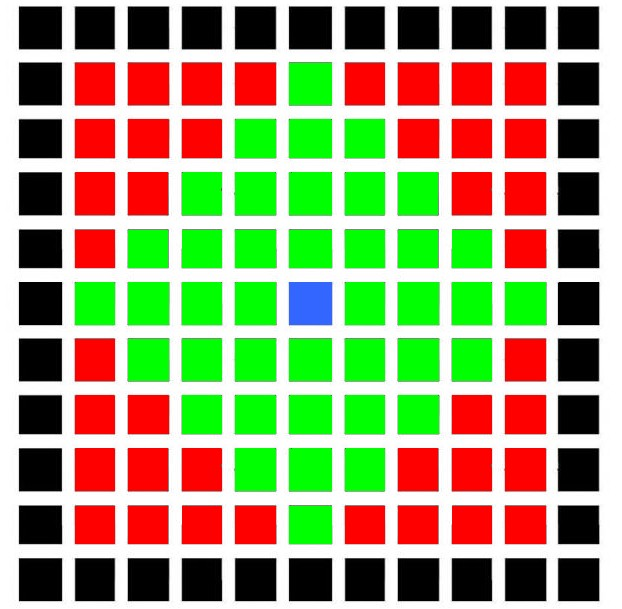
\includegraphics[width=6cm]{Images/manhattan.jpg}
	\caption{\label{manhattan} Cases à une distance Manhattan de 4}
\end{figure}

$(4)$ était également problématique puisque \mbox{\textit{Level}} et \mbox{\textit{Game}} étaient les seuls à être au courant de la réussite d'un niveau, alors que les méthodes permettant le chargement d'un niveau (via \mbox{\textit{MapParser}}) se trouvaient dans \mbox{\textit{Launcher}}. 

La solution logique semblait être de déplacer les méthodes appelant \mbox{\textit{MapParser}} de \mbox{\textit{Launcher}} vers \mbox{\textit{Game}} mais il a été décidé d'attendre la fusion des différentes extensions individuelles pour réaliser ce changement. Nous voulions en réalité éviter les conflits potentiels lors de la fusion puisque ce "transfert" de méthodes demande un nombre important de modifications dans le code d'origine. En attendant la fusion, on a donc simplement fait en sorte que \mbox{\textit{Game}} aie la référence vers une instance de \mbox{\textit{Launcher}}.

$(5)$ posait lui aussi quelques difficultés, non pas sur sa réalisation en soi mais bien sur la redondance potentielle et la future intégration avec le système de profil de l'extension \og Score \fg \, (section \ref{score}) . 

Pour cette fonctionnalité, il a été choisi de simuler l'authentification en respectant des conventions de nommage communes. On fournira ici les méthodes permettant, une fois qu'a été récupéré le niveau maximum atteint par un joueur, d'ajouter des boutons de sélection/chargement de niveau tout en réinitialisant le score et les vies du joueur.

\paragraph{Convertisseur de cartes} \label{map_generator_txt}
Pour les ajouts $(4)$ et $(5)$, il a été nécessaire d'ajouter des fichiers de niveaux supplémentaires. Puisque la démarche était fastidieuse, une fonctionnalité \og bonus \fg \, a été implémentée : la génération de fichiers de niveaux au format Pac-man à partir d'une image.

En effet, en attribuant une couleur à chaque type d'élément du jeu,  une image peut être convertie en un fichier texte équivalent et \og lisible \fg \, par \mbox{\textit{MapParser}}. Cela permet de créer des niveaux rapidement avec n'importe quel logiciel d'édition d'image puisqu'ils permettent d'utiliser des fonctionnalités comme le "remplissage" d'une zone, qui évite donc d'entrer le même caractère un grand nombre de fois (on obtient également un rendu visuel plus clair que le fichier texte équivalent). 

La figure \ref{map_generator_img} montre un exemple de résultat de conversion d'une image en son niveau équivalent dans JPacman.
\begin{figure}[h]
	\centering
	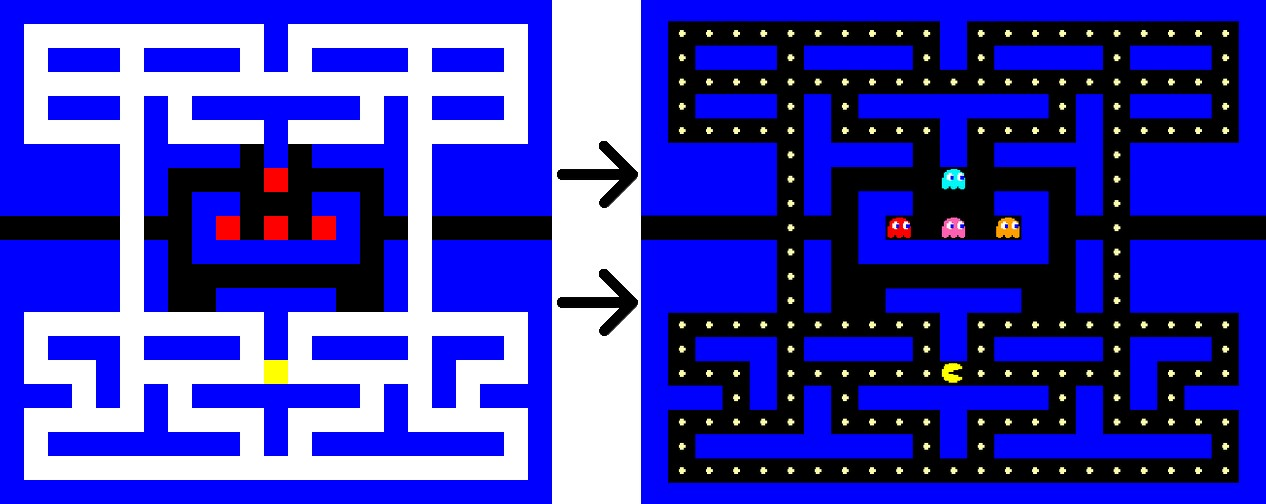
\includegraphics[width=13cm]{Images/mapgenerator.jpg}
	\caption{\label{map_generator_img} Génération d'un niveau à partir d'une image}
\end{figure}

\subsection{Fonctionnalité "IA pour Pacman"}\label{IA}

L'objectif de cette fonctionnalité est d'intégrer au code existant une intelligence artificielle pour Pacman afin qu'il puisse jouer de façon autonome tout en optimisant son score. En début de partie, le joueur doit pouvoir choisir entre contrôler Pacman manuellement ou être un spectateur passif de la partie en choisissant l'intelligence artificielle qui contrôlera Pacman à la place du joueur. Pour mettre en place cela, il a été recommandé d'utiliser un design pattern nommé "Strategy". Le design pattern "Strategy" consiste à définir un comportement (appelée "strategie") qui va permettre de différencier l'utilisation entre l'IA ou le contrôle manuel. Ce design pattern offre également une flexibilité pour modifier la stratégie suivie très facilement.

Les ajouts à effectuer pour cette extension sont les suivantes :
\begin{enumerate}
	\item Déplacement continu de Pacman,
	\item Intelligence artificielle contrôlant Pacman et qui optimise son score,
	\item Différents comportement pour Pacman,
	\item Choix du mode de jeu en début de partie (contrôle du Pacman ou spectateur passif)
	\item Extension possible et facile de nouvelles stratégies en bannissant tout type de triche \\
	
\end{enumerate} 

L'ajout de la fonctionnalité $(1)$ a été réalisé en ajoutant une méthode \mbox{\textit{Game\#continousMovement()}}, appelée à chaque fois que le joueur appuie sur une touche directionnelle, qui va manipuler un unique \textit{thread} qui va appeler, de façon périodique, la méthode \mbox{\textit{Game\#move()}}. A chaque fois que le joueur appuiera sur une touche directionnelle, la méthode \mbox{\textit{Game\#continousMovement()}} va tester si la case voulant être accédée par le joueur est accessible à Pacman. Si c'est le cas, la tâche courante du \textit{thread} est mis à jour et Pacman avance alors dans une nouvelle direction. Par contre, si ce n'est pas le cas, l'instruction est simplement ignorée et Pacman conserve alors son ancienne direction. 

\textbf{Remarque :} Pour cette fonctionnalité, il est supposé qu'il suffit d'appuyer une fois sur la touche pour conduire le Pacman dans la direction désirée ce qui veut dire que l'appui abusif d'une même touche directionnelle provoquera un ralentissement voir un arrêt du Pacman.

L'ajout de la fonctionnalité $(2)$ concerne l'implémentation d'une intelligence artificielle manipulant Pacman et qui optimise son score. Le comportement de l'IA est défini dans la classe\\
 \mbox{\textit{PacManhatanAI\#nextMove()}}. Ce comportement est calculé grâce à une recherche en largeur qui permet de déterminer la gomme la plus proche (\mbox{\textit{PacManhatanAI\#bfsNearestSafetyPelletSquare()}}). Une fois la case déterminée, il a été choisi d'utiliser un algorithme de type $A^*$ (classe \mbox{\textit{AStarPath}}
) afin de déterminer le chemin le plus court et le plus sûr en appliquant un système de poids aux cases de la carte en fonction de la présence d'une gomme, d'un fantôme ou de la proximité d'un fantôme. L'algorithme $A^*$ a été implémenté grâce à une classe template open-source fournie par Giuseppe Scrivano\footnote{http://a-star.googlecode.com/svn/trunk/java/AStar.java}
(classe \mbox{\textit{AStar}}
). Cet algorithme permet de se focaliser sur la direction du chemin en privilégiant toute direction se rapprochant de la destination par opposition à l'algorithme Dijkstra qui calcule tous les chemins possibles, ce qui est en général moins performant que l'algorithme $A^*$ car celui-ci évite autant que possible les chemins s'éloignant de la destination. Une fois un chemin déterminé, il est stocké dans une collection \textit{ArrayDeque} sous forme d'un ensemble de directions qui sera suivie par Pacman si aucun danger ne se présente (\mbox{\textit{PacManhatanAI\#convertPathToDirection()}}
). Avant de choisir le prochain mouvement, l'IA détermine si Pacman est dans une zone sûre ou non (\mbox{\textit{PacManhatanAI\#bfsNearestSafetySquare()}}
). S'il est trop proche d'un fantôme, alors l'IA choisit de prendre une nouvelle destination qui est la case sûre la plus proche. Le seuil initial pour déterminer si Pacman est proche d'un fantôme est de 14 cases, dans l'implémentation, ce qui permet de jouer un début de partie de façon très sûre. Ce seuil diminuera au cours de la partie en fonction des gommes restantes pour se focaliser sur les gommes en fin de partie (\mbox{\textit{PacManhatanAI\#updatePacmanbehaviour()}}
). Le fait d'avoir un seuil dynamique offre de bons résultats en pratique. Une fois que Pacman est dans une zone sûre, il recommence à chasser les gommes. Pour finir, pour avoir la certitude que l'IA renvoie une direction à suivre peu importe où le Pacman se trouve sur le plateau de jeu, une méthode \mbox{\textit{PacManhatanAI\#hurryMove()}}
a été implémentée pour déterminer une direction imposée qui mène à une case accessible dans le cas où aucune autre direction n'a pu être choisie. Bien que ce cas de figure n'apparaît jamais en pratique, il a été pensé en vue de l'intégration d'autres fonctionnalités comme la téléportation (voir section \ref{labyrinthe}).

\textbf{Remarque :} On peut facilement constater que l'IA se base sur la carte existante et ne passe pas par la construction d'un graphe, ce qui évite de devoir reconstruire le graphe à chaque action, ce qui pourrait être plus gourmand en performances. De plus, ce choix de comportement a été effectué en prenant en considération qu'un autre membre du projet travaillait sur un système de niveaux différents et donc les stratégies définies sur certains sites pour le jeu Pacman ne pouvaient pas être appliquées sur d'autres types de cartes. Ne pouvant pas implémenter une stratégie gagnante, il a été préféré d'appliquer une stratégie qui joue de façon la plus sûre possible tout en essayant de finir le niveau. 



L'ajout de la fonctionnalité $(3)$ a été réalisé en utilisant le design pattern "Strategy" qui va permettre d'établir différents comportement pour Pacman, sous forme de stratégie, et de choisir un type de comportement en début de partie. En ce qui concerne son implémentation, une stratégie est définie par une classe abstraite \mbox{\textit{PacmanStrategy}} qui définit certains attributs utiles aux stratégies, une méthode \mbox{\textit{PacmanStrategy\#getTypeStrategy()}} qui retourne le type de la stratégie (contrôle du Pacman par le joueur ou par une AI), une méthode \mbox{\textit{PacmanStrategy\#executeStrategy()}} qui permet d'attribuer les touches au joueur dans le cas où la stratégie choisie est le contrôle du Pacman par le joueur et une méthode \mbox{\textit{PacmanStrategy\#nextMove()}} qui retourne la prochaine direction à suivre. Une classe intermédiaire "AIStrategy" est définie pour manipuler plus facilement les stratégies où Pacman est conduit par une intelligence artificielle. Cette classe définit également des attributs plus spécifiques qui sont uniquement utiles aux stratégies de type IA pour déterminer la prochaine direction à suivre lors d'une partie en cours.

Au niveau des stratégies implémentées, la classe \mbox{\textit{HumanControllerStrategy}} représente la stratégie où le Pacman est contrôlé par un joueur humain. Le but de cette stratégie étant seulement de définir les touches de contrôle et de les attribuer au joueur pour qu'il puisse manipuler le Pacman lors d'une partie. La classe \mbox{\textit{PacManhatanAI}} représente la classe définissant le comportement de l'IA expliqué au point $(2)$.



La fonctionnalité $(4)$ a été mise en place pour que le joueur puisse choisir quelle stratégie appliquer, c'est-à-dire quel comportement attribué au Pacman pour une partie complète. Afin de laisser le joueur choisir, une fenêtre de sélection est affichée au lancement du jeu et permet de déterminer la stratégie qui sera appliquée pour toute une partie (la stratégie ne pourra pas changer lors d'un jeu en cours). Une fois que le joueur aura choisi une stratégie, il lui suffit de lancer la partie pour que celle-ci définisse un comportement spécifique à Pacman.

La classe \mbox{\textit{Level}} est utilisée pour implémenter les méthodes liées à la gestion des stratégies durant une partie. En effet, cette classe semblait la plus adéquate car elle correspond au niveau courant qui contient toutes les informations dont les stratégies ont besoin. Il est important de signaler qu'après l'intégration de toutes les fonctionnalités, les méthodes liées à la gestion des intelligences artificielles (joueur et fantômes) ont été déplacées dans une nouvelle classe \mbox{\textit{AILevel}} (voir section \ref{refactorings}). Les méthodes \mbox{\textit{Level\#start()}} et \mbox{\textit{Level\#stop()}} permettent d'exécuter ou d'arrêter l'action spécifique définie selon le type de stratégie choisie. Dans le cas d'une stratégie où le joueur est un humain, l'attribution des touches sera appliquée au joueur. Tandis que dans le cas d'une stratégie d'intelligence artificielle, la méthode \mbox{\textit{Level\#startAIStrategy()}} est appelée pour lancer un unique \textit{thread} qui va de façon périodique attribuer une direction à suivre au Pacman et appliquer un mouvement dans cette direction. Une nouvelle direction devant être calculée uniquement lorsque le Pacman se trouve à une intersection, un test a été ajouté pour définir cette situation. Dans le cas où le Pacman ne se trouve pas à une intersection, l'action effectuée correspondra à l'action courante (ancien mouvement). Le comportement du \textit{thread} pour la gestion des intelligences artificielles est défini dans la méthode \mbox{\textit{Level/PlayerMoveTask\#run()}}.


La fonctionnalité $(5)$ concerne le fait de pouvoir ajouter facilement des stratégies définissant de nouveaux comportements pour Pacman sans pour autant autoriser des stratégies qui trichent. Tout d'abord, l'implémentation des stratégies a été réfléchie pour que l'ajout de nouvelles stratégies soient faciles. En effet, comme expliqué en $(3)$, les classes abstraites \mbox{\textit{PacmanStrategy}} et \mbox{\textit{AIStrategy}} permettent de manipuler plus facilement les différents types de stratégies possibles en définissant les informations et les méthodes nécessaires aux différentes stratégies. L'implémentation d'une nouvelle stratégie se fera donc par la création d'une nouvelle classe, implémentant le comportement de la stratégie, et qui étendra l'une de ces deux classes en fonction de son type. Pour les stratégies d'intelligence artificielle, la nouvelle classe devra implémenter une méthode \mbox{\textit{nextMove()}} qui retournera la prochaine direction à suivre par Pacman. Ensuite, pour interdire tout type de triche, les attributs, se trouvant dans les classes mères \mbox{\textit{PacmanStrategy}} et \mbox{\textit{AIStrategy}}, qui représentent les caractéristiques du niveau en cours lors d'une partie, ont été implémenté avec le mot clé "final" et uniquement des méthodes d'accesseurs. Ainsi, comme les stratégies étendent ces classes, ils auront accès à ces attributs grâce aux méthodes accesseurs mais ne pourront en aucun cas modifier ces valeurs. En ne permettant pas de modifier les données du jeu, les stratégies ne pourront pas tricher dans la manipulation des données lors du calcul de la prochaine direction à suivre.

\section{Conflits et solutions lors de l'intégration}

Cette section met en avant les problèmes de conflits rencontrés lors de l'intégration des extensions individuelles (voir section \ref{extensions}) ainsi que les solutions qui ont été apportées à ces problèmes.

La liste non exhaustive suivante présente les principaux conflits qui ont été rencontrés :\\
\begin{itemize}
\item Incohérence au niveau de la documentation de certaines méthodes causée par l'assemblage de plusieurs documentations différentes lors de l'intégration.

\item Problèmes de conflits liés à l'ajout ou la suppression d'accolades et d'importations dans le code.

\item Conflits entre deux extensions ayant des comportements différents dans une même situation. Par exemple, une extension présentait un jeu où le joueur avait une seule vie tandis que l'autre présentait un jeu où le joueur avec trois vies, ce qui a conduit à des problèmes dans le cas où le joueur mourait.

\item Problèmes de dysfonctionnement au niveau de certaines fonctionnalités causés par un conflit avec une autre extension. Par exemple, des problèmes ont été rencontrées entre l'intelligence artificielle et le systèmes de plusieurs niveaux.

\item Incohérence au niveau des paramètres et du corps de certaines méthodes causée par l'assemblage de plusieurs méthodes différentes ayant le même nom dans le code.

\item Dysfonctionnement de certains tests unitaires qui devaient être adaptés aux comportements des autres extensions.
\item Problèmes de gestion de fichiers (création et écriture) lié au fait que certaines extensions ont été développé sur des systèmes d'exploitation différents.
\item ...
\end{itemize}

Avant de présenter les solutions apportées aux différents problèmes de conflits rencontrés, il faut savoir que la plupart des conflits ont été résolus par \textit{Kdiff3}\footnote{http://kdiff3.sourceforge.net/} qui est un analyseur graphique de différence des textes. Ce logiciel permet d'identifier les différences au sein des textes, ou parmi les fichiers et  nous informe lorsqu'il y a eu des modifications.

La liste non exhaustive suivante présente les principales solutions qui ont été apportées :\\
\begin{itemize}
\item Adaptation de certains paramètres de méthodes pour pouvoir intégrer les fonctionnalités ensemble.
\item Adaptation du processus de victoire et de défaite lié aux niveaux et aux vies.
\item Adaptation du système de gestion de fichier pour qu'il puisse fonctionner sur tout système d'exploitation.
\item Adaptation de certains tests unitaires.
\item Adaptation du comportement de l'IA pour un jeu contenant plusieurs niveaux.
\item ...
\end{itemize}

Il est également important de signaler que l'étape d'intégration a été réalisée assez facilement grâce à d'importantes discussions, au préalable, concernant les choix d'implémentations qui ont permises de faciliter l'intégration en minimisant les conflits.


\section{Refactorings avant analyse}\label{refactorings}
Cette section présente les \textit{refactorings} qui ont été effectués avant que des outils d'analyse n'aient été utilisés. Certaines ont d'ailleurs été
planifiées avant la fusion des versions individuelles mais n'ont pas été réalisées dans l'immédiat pour limiter le nombre de conflits avec les autres versions lors de l'intégration des \og pull requests \fg .

\paragraph{Déplacement de la variable retenant le niveau courant de \textit{Level} vers \textit{Game} : }
Ce placement semble plus logique et évite un problème de \og feature envy \fg de méthodes de \mbox{\textit{Game}} y accédant.
\paragraph{Déplacement des méthodes concernant le \og map parser \fg \, de \textit{Launcher} vers \textit{Game} : }
Cette nouvelle organisation semble plus logique et évite que \mbox{\textit{Game}} ne doive avoir une référence vers le \mbox{\textit{Launcher}} qui l’a créé (pour pouvoir charger le niveau suivant en cas de victoire).
Cela a cependant nécessité de passer des méthodes/variables en \og static \fg \, : une partie des \og accesseurs \fg \, aux \og Factories \fg \, de \mbox{\textit{Launcher}}, puisque \mbox{\textit{MapParser}} en a besoin. Cette modification reste malgré tout logique puisque ces méthodes/variables sont en effet uniques au runtime.

\paragraph{Déplacement de la gestion des IA de la classe \textit{Level} vers \textit{AILevel} : } Ce déplacement permet de regrouper toutes les méthodes liées aux IA (joueurs et fantômes) au sein d'une unique classe. Cette classe héritant de la classe \textit{Level} permet d'avoir toujours accès aux informations du niveau courant dont les IA ont besoin pour fonctionner. Ce \textit{refactoring} a été appliqué dans le but de réduire la classe \textit{Level} qui devenait trop complexe et de localiser la gestion des IA au sein d'une classe pour faciliter l'évolution du logicielle et sa maintenance.

\section{Analyse de la qualité du code source}

Dans cette section, nous allons comparer la qualité du code source qui intègre toutes les extensions individuelles avec la qualité du code source de la version de départ de JPacman. Pour pouvoir effectuer cette comparaison, il va, tout d'abord, falloir effectuer des analyses sur la qualité du code source des deux versions en utilisant différentes techniques. Pour faire cela, nous ferons appel à plusieurs outils d'analyse de qualité que nous détaillerons par la suite. Cette phase se déroulera en deux étapes : une analyse statique et une analyse dynamique du code. Cette analyse doit permettre de comprendre la structure du logiciel et de situer les parties du code pouvant causer problème.

\subsection{Analyse statique}

\subsubsection{Métriques}

Dans cette section, nous allons analyser la qualité du logiciel initial ainsi que la qualité du logiciel après intégration des extensions, grâce à des métriques, afin de comparer les deux versions. Un ensemble de métriques logiciels peut être calculé pour mesurer la qualité interne du logiciel. Ces métriques peuvent ainsi être utilisées pour identifier les problèmes liés à la qualité des systèmes logiciels existant. Il existe un grand nombre de catégories de métriques telles que les métriques de taille, de cohésion et de couplage, de dépendance, de complexité ou encore de similarité. Pour ce projet, l'ensemble des métriques est calculé par le biais d'un plugin de l'IDE Intellij Idea qui s'appelle \textit{Metrics Reloaded} (version 1.6.1). Ce plugin permet d'obtenir des informations concernant un grand nombre de métriques sur un projet. \\

\subsubsection*{\textbf{\large{1) Métrique de taille}}}


Les métriques de taille sont les métriques statiques les plus simples à définir, comprendre et calculer. Elles donnent une idée de la taille du logiciel, en calculant par exemple le nombre de lignes de code source dans les classes, le nombre de classes dans les paquets,... Généralement les
métriques de taille sont utilisées pour comparer la taille de différents logiciels, pour prévoir les efforts de développement et de maintenance.\\

\textbf{a) Nombre de classes}

Cette métrique fournit des informations concernant la distribution des classes au sein du projet en donnant le nombre total de classes (en prenant en compte les interfaces) par package. 

\textbf{Logiciel initial}

Les résultats obtenus sont reportés dans les figures suivantes (Figures~\ref{classMetrics1} et \ref{classMetrics2}) où la colonne \textit{C} représente le nombre de classes et d'interfaces dans chaque package et la colonne \textit{C(rec)} représente le nombre de classes et d'interfaces dans chaque package en incluant les sous-classes. Les autres colonnes concernent la distribution des classes au sein du code produit et du code de test.

\begin{figure}[!h]
	\centering
	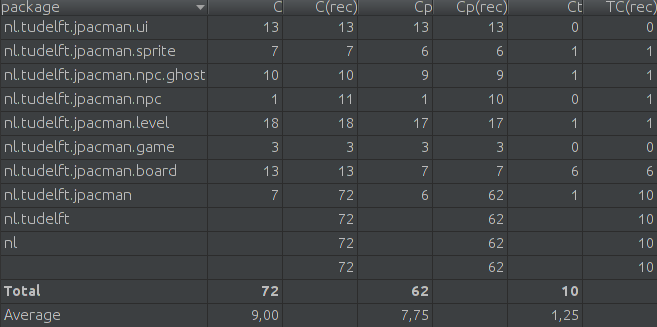
\includegraphics[scale=0.6]{Images/classMetrics1.png} 
	\caption{Nombre de classes et d'interfaces dans chaque package}
	\label{classMetrics1}
\end{figure}

\begin{figure}[!h]
	\centering
	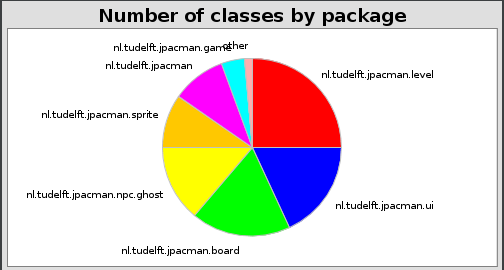
\includegraphics[scale=0.7]{Images/classMetrics2.png} 
	\caption{Répartition graphique des classes au sein des packages}
	\label{classMetrics2}
\end{figure}
\newpage
\textbf{Logiciel final}

Effectuons cette analyse sur le logiciel final, c'est-à-dire le logiciel qui contient la version après intégration des fonctionnalités.

\begin{figure}[!h]
	\centering
	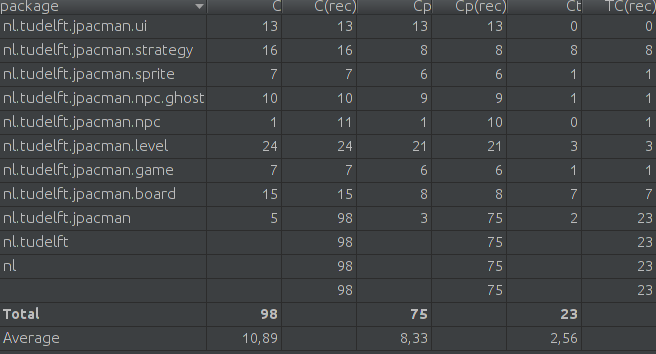
\includegraphics[scale=0.6]{Images/classMetrics3.png} 
	\caption{Nombre de classes et d'interfaces dans chaque package}
	\label{classMetrics3}
\end{figure}

\begin{figure}[!h]
	\centering
	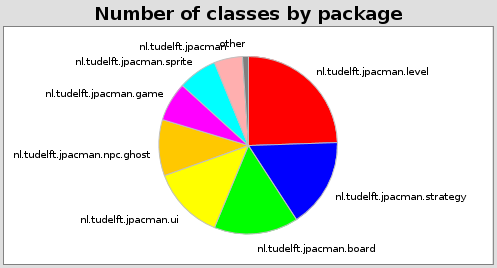
\includegraphics[scale=0.7]{Images/classMetrics4.png} 
	\caption{Répartition graphique des classes au sein des packages}
	\label{classMetrics4}
\end{figure}
\newpage
Après l'ajout d'un nouveau package (strategy) et de nouvelles classes, on constate que la distribution des classes au sein des packages n'a pas beaucoup changé avec une moyenne de 2 classes (ou interfaces) en plus par package (Figure~\ref{classMetrics3} et \ref{classMetrics4}).\\


\textbf{b) Lignes de codes}


Cette métrique permet de détecter les classes volumineuses qui peuvent être à l'origine d'une grande complexité. Elle permet également de détecter d'éventuelles "god class".

\textbf{Logiciel initial}

Dans un premier temps, on peut analyser le nombre de lignes de code à l'intérieur de chaque package (Figure~\ref{locinit}) en ne considérant pas les classes de tests. On constate ainsi une moyenne de 482 lignes de codes par package. Le package le plus volumineux semble être le package "Level" qui contient 1183 lignes de codes. Ce n'est pas très étonnant car ce package a été analysé comme étant celui qui contient le plus de classes (voir métrique "Nombre de classes"). On peut aussi observer qu'il y a, au total, 3860 lignes de codes si on inclus les lignes de commentaires et 1905 lignes de code java sans les commentaires (Figure~\ref{locinit2}).

\begin{figure}[!h]
	\centering
	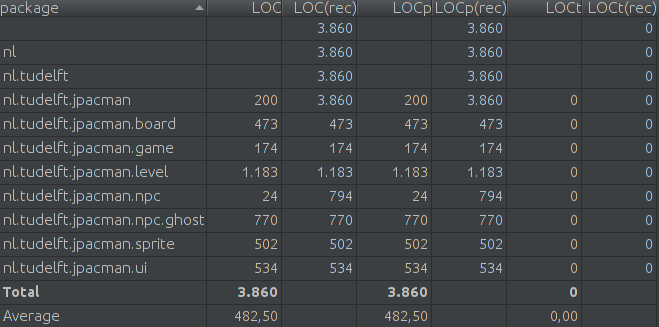
\includegraphics[scale=0.6]{Images/SizeMetricsLOC.png} 
	\caption{Nombre de lignes de code dans chaque package}
	\label{locinit}
\end{figure}





\begin{figure}[!h]
	\centering
	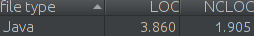
\includegraphics[scale=0.6]{Images/SizeMetricsLOC2.png} 
	\caption{Nombre de lignes de code avec et sans les commentaires}
	\label{locinit2}
\end{figure}

\newpage
Ensuite, grâce au plugin "Statistic" de l'IDE Intellij Idea, on peut afficher plus en détail les statistiques concernant les lignes de code dans le projet (en prenant en compte les classes de tests). Dans les résultats dans la figure~\ref{locinit3}, on constate que la classe la plus volumineuse est la classe \mbox{\textit{Level}}.

\begin{figure}[!h]
	\centering
	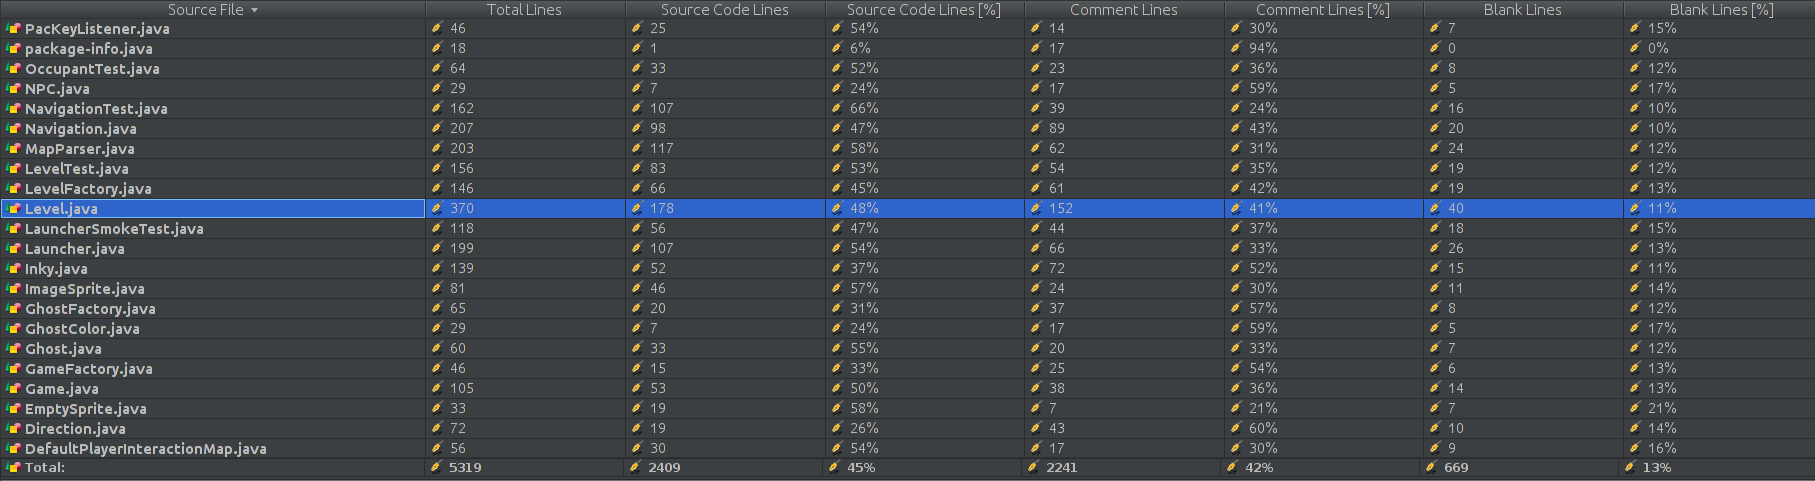
\includegraphics[scale=0.29]{Images/SizeMetricsLOC3.png} 
	\caption{Statistiques sur les lignes de codes}
	\label{locinit3}
\end{figure}



\textbf{Logiciel final}

Concernant la version finale, les résultats de la distribution des lignes de codes dans les packages sont reportés dans les figures~\ref{locfinal} et \ref{locfinal2}. Ces résultats montrent que le package "Level" reste le plus volumineux de tous et le nombre moyen de lignes de code par package a augmenté de 482 à 720. Quant au nombre de lignes de code total, il est passé de 3860 à 6487 et de 1905 à 3503 si on ne compte pas les commentaires.

\begin{figure}[!h]
	\centering
	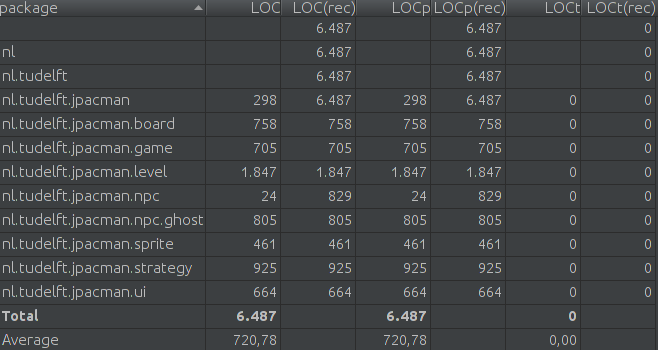
\includegraphics[scale=0.6]{Images/SizeMetricsLOCFinal.png} 
	\caption{Nombre de lignes de code dans chaque package}
	\label{locfinal}
\end{figure}
\begin{figure}[!h]
	\centering
	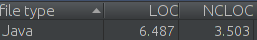
\includegraphics[scale=0.6]{Images/SizeMetricsLOCFinal2.png} 
	\caption{Nombre de lignes de code avec et sans les commentaires}
	\label{locfinal2}
\end{figure}
\newpage
Quant aux statistiques (Figure~\ref{locfinal3}), on constate que les deux classes les plus volumineuses sont \mbox{\textit{IdentifiedPlayer}} et  \mbox{\textit{Level}}. On constate également que la plupart des valeurs totales des statistiques ont été doublées par rapport à la version originale.


\begin{figure}[!h]
	\centering
	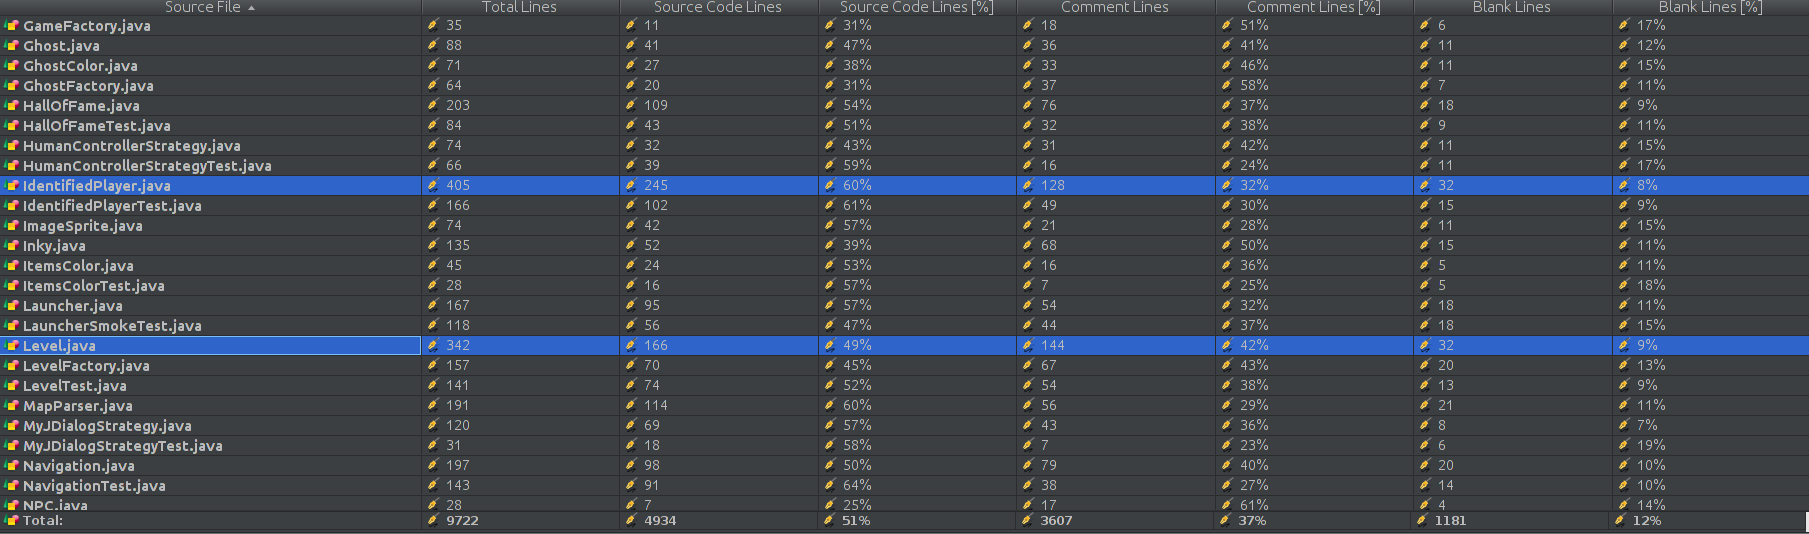
\includegraphics[scale=0.29]{Images/SizeMetricsLOCFinal3.png} 
	\caption{Statistiques sur les lignes de codes}
	\label{locfinal3}
\end{figure}
\subsubsection*{\textbf{\large{2) Métrique de complexité}}}

Ces métriques sont utilisées pour mesurer la complexité d’une partie du logiciel. Elles sont souvent corrélées avec les métriques de taille parce qu’un très grand système a de grandes chances d’être également complexe.\\

\textbf{a) Complexité}


Cette métrique permet de calculer la complexité cyclomatique des différentes classes du projet. La complexité cyclomatique d'une fonction peut être définie comme le nombre de chemins d'exécutions possible dans cette fonction, ce qui est fortement influencé par la présence de boucles ou de conditions dans celle-ci. La complexité cyclomatique d'une méthode vaut au minimum 1, puisqu'il y a toujours au moins un chemin. Au niveau de l'interprétation, la complexité cyclomatique d'une méthode augmente proportionnellement au nombre de points de décision, ce qui signifie qu'une méthode avec une haute complexité est plus difficile à comprendre et à maintenir. En général, une complexité cyclomatique trop élevée indique qu'il faut refactoriser la méthode. Par contre, si une méthode a une complexité convenable (en dessous d'un certain seuil), elle peut être acceptable si elle est suffisamment testée. Cette métrique est liée à la métrique de couverture du code par les tests. En effet, une méthode devrait avoir un nombre de tests unitaires égal à sa complexité cyclomatique pour avoir un "code coverage" de $100\%$, ainsi chaque chemin de la méthode est testé.

\textbf{Logiciel initial}

Les figure~\ref{ComplexityMetrics1} et \ref{ComplexityMetrics2}  mettent en évidence les classes et les méthodes possédant une complexité au-dessus d'un certain seuil (les classes ou méthodes en dessous du seuil ne sont pas représentées par souci de lisibilité). Cette analyse nous permet de mettre en évidence que certaines classes ou méthodes sont potentiellement complexes par rapport aux autres au sein du projet. Elles doivent donc être surveillées de près dans les analyses du logiciel final.


\begin{figure}[!h]
	\centering
	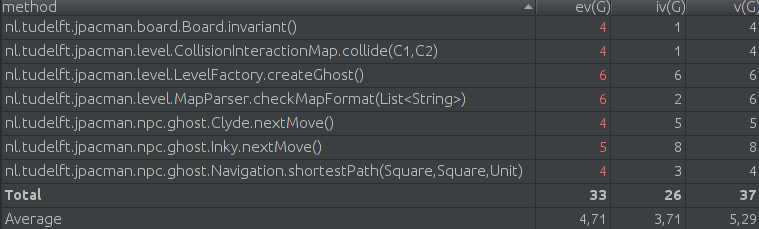
\includegraphics[scale=0.6]{Images/ComplexityMetrics1.png} 
	\caption{Métrique de complexité pour les méthodes}
	\label{ComplexityMetrics1}
\end{figure}


\begin{figure}[!h]
	\centering
	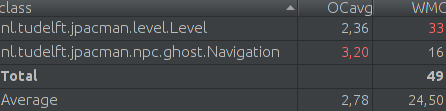
\includegraphics[scale=0.6]{Images/ComplexityMetrics2.png} 
	\caption{Métrique de complexité pour les classes}
	\label{ComplexityMetrics2}
\end{figure}
\newpage
\textbf{Logiciel final}

Les figure~\ref{ComplexityMetrics3} et \ref{ComplexityMetrics4}  mettent en évidence ces métriques pour la version finale du logiciel. En observant ces valeurs, on peut en déduire que la complexité de ces méthodes reste acceptable car chaque méthode ajoutée lors des extensions a fait l'objet de tests unitaires. En observant ces résultats, on constate que très peu de méthodes, par rapport au nombre de méthodes qui ont été rajoutés avec les trois extensions, ont une complexité trop élevée. De plus, la plupart de ces méthodes interviennent dans la gestion de l'intelligence artificielle manipulant Pacman. Vu que ces méthodes utilisent beaucoup d'information et un grand nombre de possibilités différentes, il n'est pas étonnant que leur complexité soit plus élevée. Malgré tout, ces méthodes ont fait l'objet de tests unitaires permettant de valider leurs comportements.

\begin{figure}[!h]
	\centering
	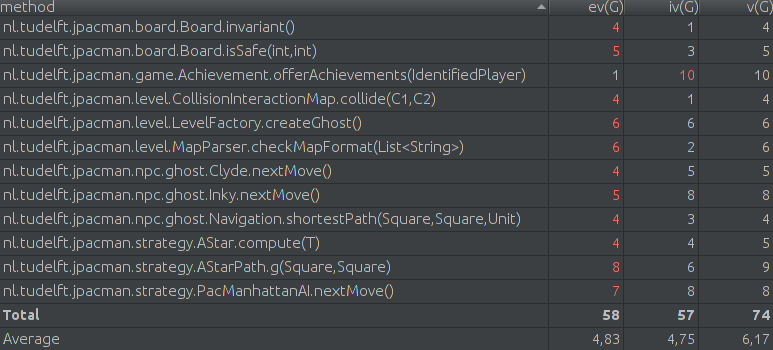
\includegraphics[scale=0.6]{Images/ComplexityMetrics3.png} 
	\caption{Métrique de complexité pour les méthodes}
	\label{ComplexityMetrics3}
\end{figure}


\begin{figure}[!h]
	\centering
	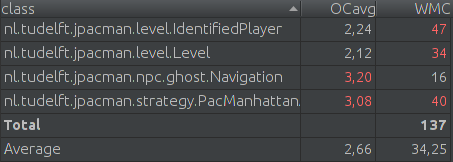
\includegraphics[scale=0.6]{Images/ComplexityMetrics4.png} 
	\caption{Métrique de complexité pour les classes}
	\label{ComplexityMetrics4}
\end{figure}


\newpage

\subsubsection*{\textbf{\large{3) Métrique de couplage et de cohésion}}}



Les métriques de couplage décrivent les dépendances entre les composants du système. Plus le couplage entre deux composants est fort, plus le système est compliqué à comprendre, modifier ou corriger.


Les métriques de cohésion décrivent le taux de connectivité au sein d’un composant du
logiciel. Celle-ci mesure donc le taux d’utilisation des attributs d’une classe par les méthodes de cette même classe et mesure donc l’application des principes d’encapsulation des données. C’est un facteur important pour la portabilité, la fiabilité et donc pour la qualité globale du système. Une forte cohésion engendre un couplage faible, ce qui signifie que les deux métriques sont donc corrélées entre elles.\\

\textbf{a) Couplage et cohésion}


L'analyse de couplage peut se faire via la métrique CBO (\textit{coupling between object classes}) qui permet de mesurer le nombre d'autres classes couplées à une classe donnée. En effet, CBO représente le couplage en comptant le nombre de classes différentes rattachées à une classe précise autant en entrée qu'en sortie.

En ce qui concerne l'analyse de la cohésion des classes, la métrique LCOM (\textit{Lack of Cohesion in Methods}) peut être utilisée pour mesurer la cohésion entre les méthodes d'une classe. Cette métrique représente le manque de cohésion au sein d'une classe (une grande valeur pour cette métrique représente un manque de cohésion dans cette classe).

\textbf{Logiciel initial}

Par souci de lisibilité dans ce rapport, nous afficherons seulement une partie des classes du projet pour visualiser leurs couplages et leurs cohésions. La figure~\ref{MetricsCohesion1} affiche une moyenne de $8.78$ pour la métrique CBO et $1.58$ pour la métrique LCOM du projet. 


On constate également une valeur moyenne de $2.02$ pour la métrique DIT (\textit{Depth Inheritence Tree}) qui sert de mesure structurelle sur la hiérarchie des classes du systèmes. Pour une classe donnée, DIT représente la longueur du chemin pour se rendre de la racine à cette classe en passant par les liens d'héritage.

Et pour finir, on observe une valeur moyenne de $7.73$ pour la métrique WMC (\textit{Weighted Methods per Class}) qui sert de mesure de taille et de complexité puisqu'elle additionne le nombre de méthodes d'une classe pondéré par un facteur de complexité quelconque.

\begin{figure}[!h]
	\centering
	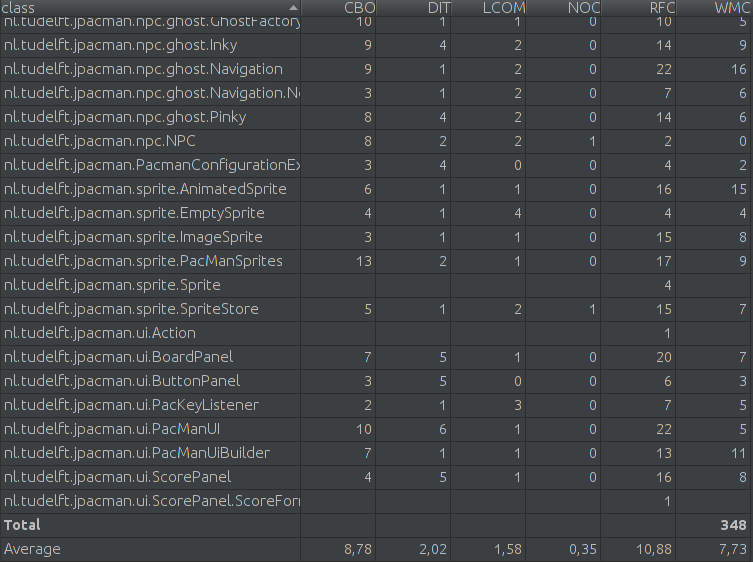
\includegraphics[scale=0.6]{Images/MetricsCohesion1.png} 
	\caption{Métriques de cohesion et couplage}
	\label{MetricsCohesion1}
\end{figure}

\newpage
\textbf{Logiciel final}

Effectuons cette même analyse sur la version finale où les résultats sont reportés dans la figure~\ref{MetricsCohesion2}. On observe que la moyenne de la métrique CBO du projet est désormais de $10.63$ contre $8.78$ dans la version initiale. La valeur moyenne de la métrique LCOM du projet est maintenant de $1.83$ contre $1.58$ précédemment. La métrique DIT atteint la valeur moyenne de $1.98$ contre $2.02$. Pour terminer, la moyenne de la métrique WMC du projet est désormais de $10.14$ contre $7.73$ dans la version initiale.

Mise à part la métrique DIT, on constate que les métriques de cohésion et de couplage ont légèrement augmenté par rapport à la version initiale. Ces résultats ne sont pas étonnant car avec l'ajout de trois extensions qui ont modifié considérablement le jeu initial, il est normal que les couplages et cohésions entre classes augmentent ne serait-ce que légèrement.

\begin{figure}[!h]
	\centering
	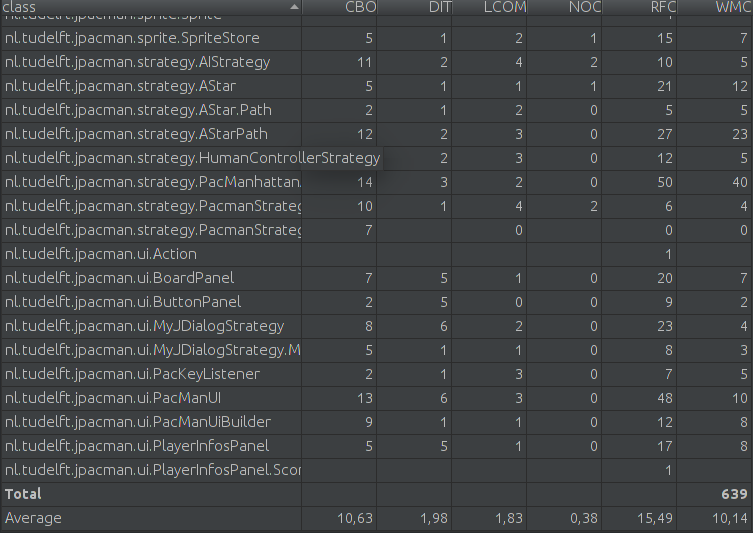
\includegraphics[scale=0.6]{Images/MetricsCohesion2.png} 
	\caption{Métriques de cohesion et couplage}
	\label{MetricsCohesion2}
\end{figure}

\newpage
\textbf{b) Dépendance}


Cette métrique permet de connaître les différentes dépendances entre classes. Ces dépendances doivent toujours être plus ou moins faibles afin de garder une bonne modularité du logiciel.

\textbf{Logiciel initial}

Par souci de lisibilité dans ce rapport, nous afficherons seulement une partie des classes du projet pour visualiser leurs dépendances. La figure~\ref{DependencyMetrics1} montre que les dépendances sont relativement correcte.

\begin{figure}[!h]
	\centering
	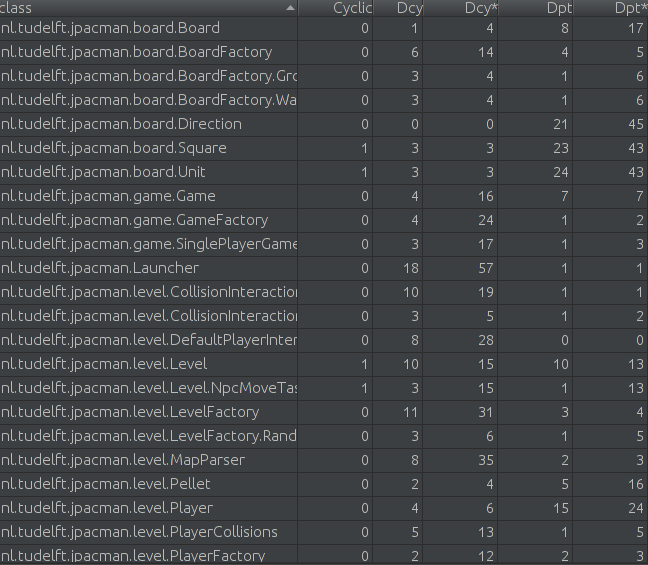
\includegraphics[scale=0.5]{Images/DependencyMetrics1.png}
	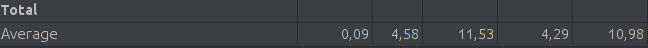
\includegraphics[scale=0.5]{Images/DependencyMetricsBis1.png}  
	\caption{Métrique de dépendance}
	\label{DependencyMetrics1}
\end{figure}
\newpage
 On peut également s’intéresser à la dépendance cyclique, une métrique qui met en évidence les classe dépendantes l'une de l'autre. Les différentes classes possédant une dépendance cyclique sont représentées dans la figure~\ref{DependencyCycle1}. En analysant le fonctionnement de ces différentes classes, on remarque que leur interdépendance est plutôt logique. Par exemple, il est normale que les classes du package "ghost" soient liées aux classes du package "sprite" car les fantômes sont représentés visuellement dans le jeu.





\begin{figure}[!h]
	\centering
	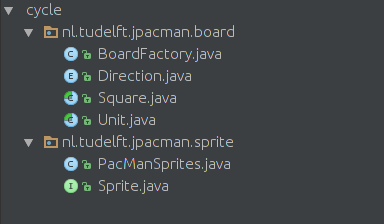
\includegraphics[scale=0.5]{Images/DependencyCycle1.png}
	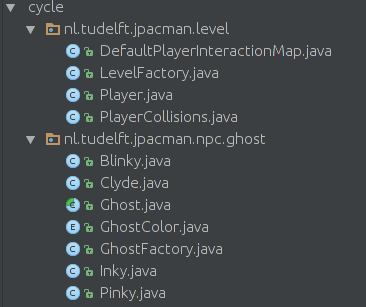
\includegraphics[scale=0.5]{Images/DependencyCycle2.png}  
\end{figure}

\begin{figure}[!h]
	\centering
	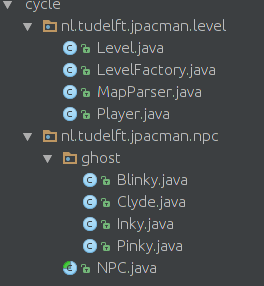
\includegraphics[scale=0.5]{Images/DependencyCycle3.png}
	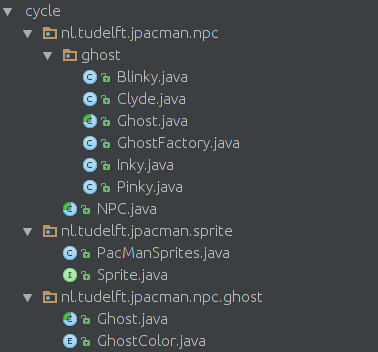
\includegraphics[scale=0.5]{Images/DependencyCycle4.png}  
\end{figure}

\begin{figure}[!h]
	\centering
	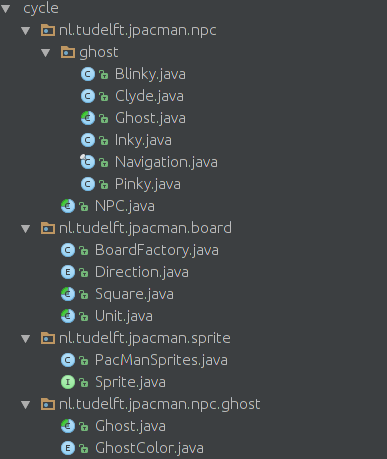
\includegraphics[scale=0.4]{Images/DependencyCycle5.png}
	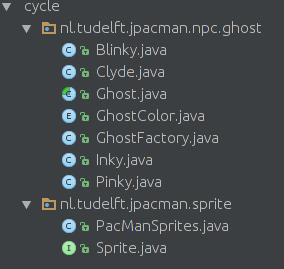
\includegraphics[scale=0.5]{Images/DependencyCycle6.png} 
		\caption{Dépendances cycliques}
 
	\label{DependencyCycle1}
\end{figure}

\newpage

La matrice de dépendance qui est représentée par la figure~\ref{DependencyMatrix1} permet de mieux visualiser ces dépendances entre classes. Dans cette matrice, les cases bleues représentent les dépendances unidirectionnelles tandis que les cases rouges représentent les dépendances bidirectionnelles (cycles). Il est donc conseillé d'éviter au maximum les cycles.

\begin{figure}[!h]
	\centering
	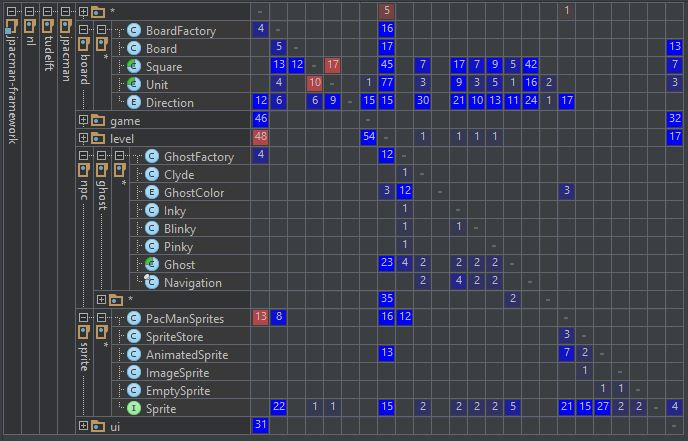
\includegraphics[scale=0.5]{Images/DependencyMatrix1.JPG}
	\caption{Matrice de dépendances}
	\label{DependencyMatrix1}
\end{figure} 



\textbf{Logiciel final}

Encore une fois, seule une partie des classes seront affichées par souci de lisibilité dans le rapport. La figure~\ref{DependencyMetricsFinal1} montre les dépendances entre les classes après intégration des trois fonctionnalités. On peut facilement observer que le nombre de dépendances a fortement augmenté.

\begin{figure}[!h]
	\centering
	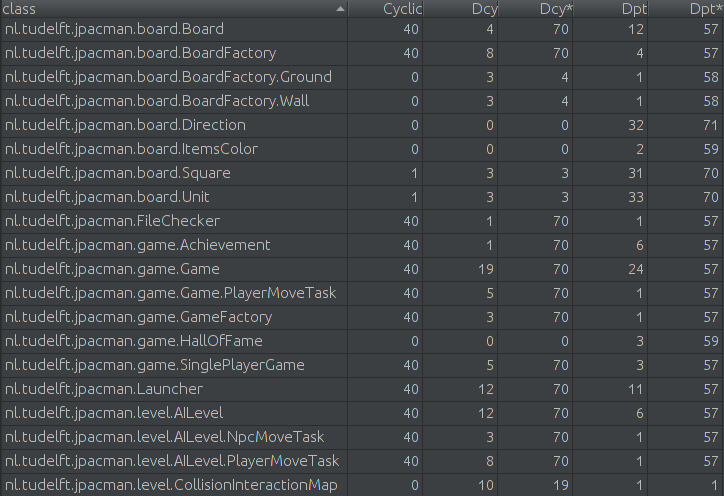
\includegraphics[scale=0.6]{Images/MetricsDependencyFinal1.png}  
	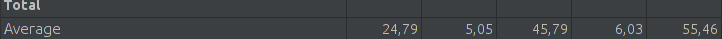
\includegraphics[scale=0.6]{Images/MetricsDependencyFinal2.png} 
	\caption{Métrique de dépendance}
	\label{DependencyMetricsFinal1}
\end{figure}

\newpage


Si on analyse les dépendances cycliques entre les packages, on constate qu'elles ont elles aussi augmenté considérablement. Les figures~\ref{CyclicDependencyFinal1} à \ref{CyclicDependencyFinal8} représentent les dépendances cycliques entre les différentes classes des packages.

\begin{figure}[!h]
	\centering
	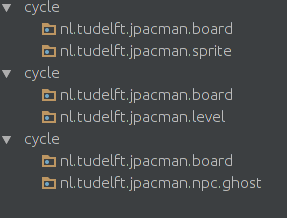
\includegraphics[scale=0.6]{Images/CyclicDependencyFinal1.png}  
		\caption{Dépendances cycliques pour le package \textit{board}}
	\label{CyclicDependencyFinal1}
\end{figure}

\begin{figure}[!h]
	\centering
	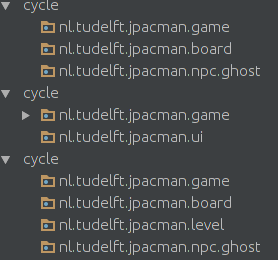
\includegraphics[scale=0.6]{Images/CyclicDependencyFinal2.png} 
	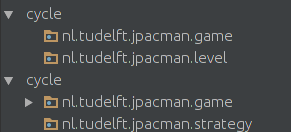
\includegraphics[scale=0.6]{Images/CyclicDependencyFinal3.png}   
		\caption{Dépendances cycliques pour le package \textit{game}}
	\label{CyclicDependencyFinal2}
\end{figure}

\begin{figure}[!h]
	\centering
	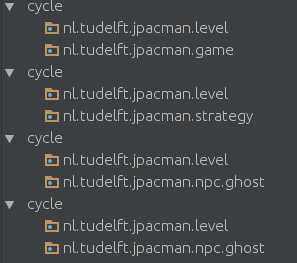
\includegraphics[scale=0.6]{Images/CyclicDependencyFinal4.png} 
	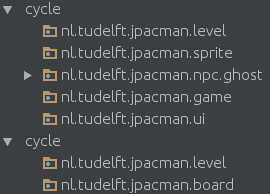
\includegraphics[scale=0.6]{Images/CyclicDependencyFinal5.png}   
		\caption{Dépendances cycliques pour le package \textit{level}}
	\label{CyclicDependencyFinal3}
\end{figure}

\begin{figure}[!h]
	\centering
	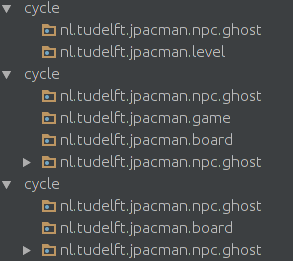
\includegraphics[scale=0.6]{Images/CyclicDependencyFinal7.png} 
	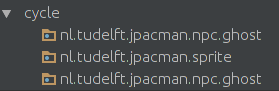
\includegraphics[scale=0.6]{Images/CyclicDependencyFinal8.png}   
		\caption{Dépendances cycliques pour le package \textit{npc}}
	\label{CyclicDependencyFinal4}
\end{figure}

\begin{figure}[!h]
	\centering
	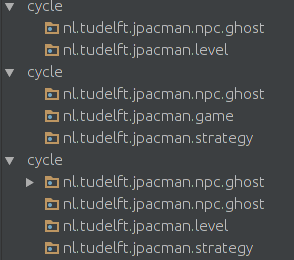
\includegraphics[scale=0.6]{Images/CyclicDependencyFinal9.png} 
	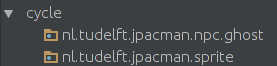
\includegraphics[scale=0.6]{Images/CyclicDependencyFinal10.png}   
		\caption{Dépendances cycliques pour le package \textit{npc.ghost}}
	\label{CyclicDependencyFinal5}
\end{figure}

\begin{figure}[!h]
	\centering
	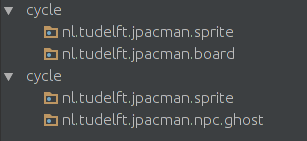
\includegraphics[scale=0.6]{Images/CyclicDependencyFinal11.png}    
		\caption{Dépendances cycliques pour le package \textit{sprite}}
	\label{CyclicDependencyFinal6}
\end{figure}

\begin{figure}[!h]
	\centering
	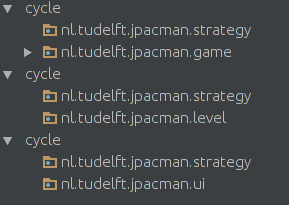
\includegraphics[scale=0.6]{Images/CyclicDependencyFinal12.png}    
		\caption{Dépendances cycliques pour le package \textit{strategy}}
	\label{CyclicDependencyFinal7}
\end{figure}

\begin{figure}[!h]
	\centering
	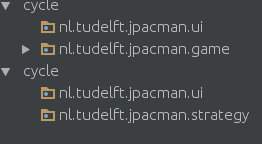
\includegraphics[scale=0.6]{Images/CyclicDependencyFinal13.png}    
		\caption{Dépendances cycliques pour le package \textit{ui}}
	\label{CyclicDependencyFinal8}
\end{figure}




\newpage

La matrice de dépendance qui est représentée par la figure~\ref{DependencyMatrix2} permet de mieux visualiser ces dépendances entre classes. On observe assez facilement que le nombre de dépendances cycliques a augmenté par rapport à la version initiale. Encore une fois, ce résultat peut être expliqué par l'ajout de nombreuses modifications par rapport à cette version. En effet, la version initiale implémente un jeu très basique avec une seule fonctionnalité (un mode de jeu sur un niveau) tandis que la version finale implémente un jeu plus "élaboré" contenant plusieurs fonctionnalités (plusieurs modes de jeu et niveaux,...). Il est donc évident que cette amélioration a un impact direct sur les dépendances entre classes car les fonctionnalités ajoutées interagissent ensemble. On peut donc en conclure que ces résultats sont tout à fait convenables et cohérents si on prend en considération l'ampleur des modifications qui ont été effectuées.

\begin{figure}[!h]
	\centering
	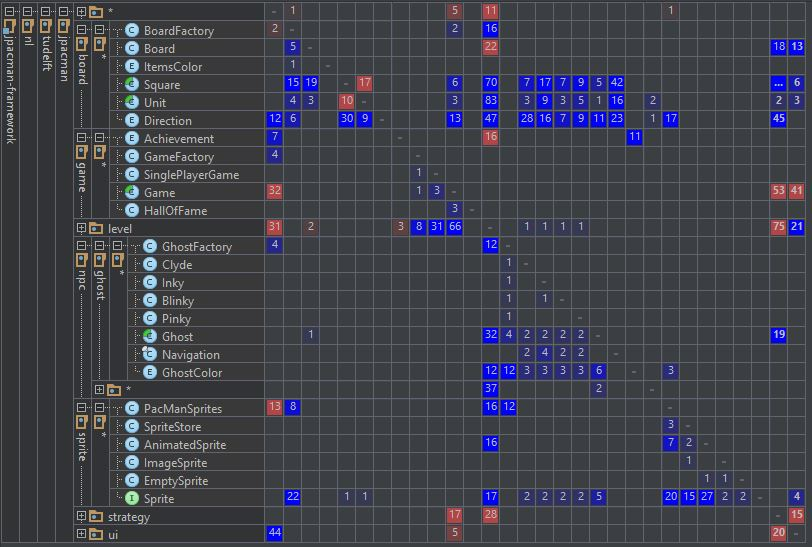
\includegraphics[scale=0.5]{Images/DependencyMatrix2.JPG}
	\caption{Matrice de dépendances}
	\label{DependencyMatrix2}
\end{figure} 

\subsubsection*{\textbf{\large{Analyse de SonarQube}}}

Avant de terminer cette analyse au niveau des métriques, le logiciel \textit{SonarQube} a été utilisé pour avoir les résultats d'un autre logiciel d'analyse de qualité du code. \textit{SonarQube} est un outil tout-en-un, indépendant des IDEs, qui permet de calculer et monitorer la qualité logicielle, de voir l'évolution entre les versions du logiciel et aussi de comparer ces versions entre elles très facilement. C'est un outil open source qui a pour objectif de fournir une analyse complète de la qualité d'une application en fournissant de nombreuses statistiques (ou métriques) sur un projet. Ces données permettent d'évaluer la qualité du code, et d'en connaître l'évolution au cours du développement.


Nous pouvons ainsi encore une fois comparer les résultats obtenus (pour certaines métriques) pour la version finale avec le version initiale. Il est important de spécifier que les métriques utilisés par ce logiciel ne sont pas nécessairement les mêmes que celles utilisées précédemment, ce qui implique que les résultats ne sont pas exactement les mêmes que lors des analyses précédentes.
\newpage
\textbf{Logiciel initial}

Effectuons une analyse de certaines métriques sur la version initiale dont on a reporté les résultats dans les figures~\ref{sonarInitial1} à ~\ref{sonarInitial4}.

\begin{figure}[!h]
	\centering
	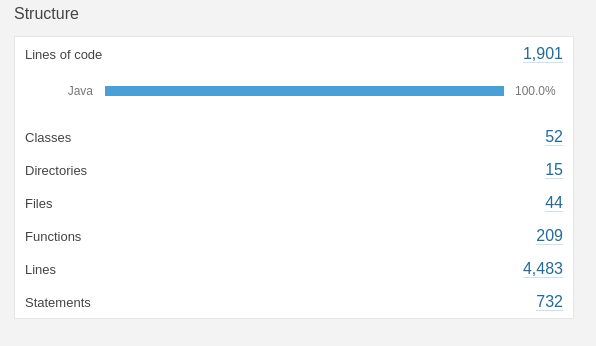
\includegraphics[scale=0.5]{Images/sonarInitial1.png} 
	\caption{Caractéristique de la structure}
	\label{sonarInitial1}
\end{figure} 

\begin{figure}[!h]
	\centering
	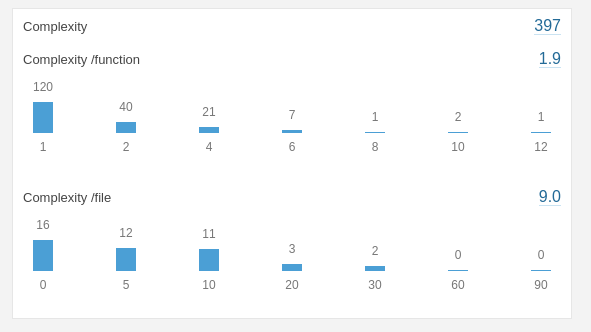
\includegraphics[scale=0.5]{Images/sonarInitial2.png} 
	\caption{Caractéristique de la complexité}
	\label{sonarInitial2}
\end{figure} 

\begin{figure}[!h]
	\centering
	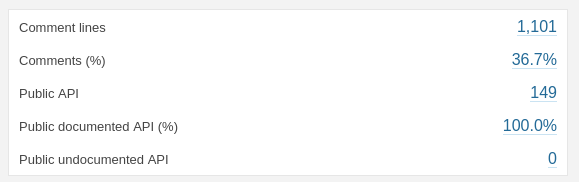
\includegraphics[scale=0.5]{Images/sonarInitial3.png} 
	\caption{Pourcentages des commentaires et de la documentation}
	\label{sonarInitial3}
\end{figure} 

\begin{figure}[!h]
	\centering
	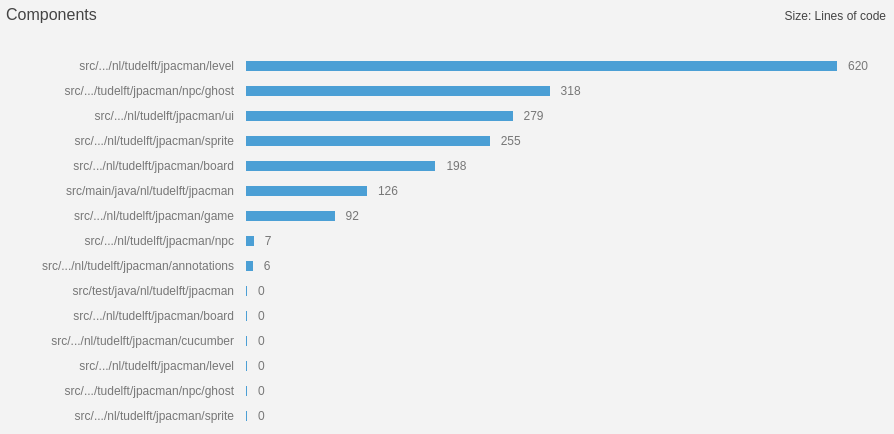
\includegraphics[scale=0.5]{Images/sonarInitial4.png} 
	\caption{Répartition des lignes de codes}
	\label{sonarInitial4}
\end{figure} 


\newpage
\textbf{Logiciel final}

Effectuons, à présent, la même analyse avec la version finale dont on a reporté les résultats dans les figures~\ref{sonarFinal1} à ~\ref{sonarFinal4}.


\begin{figure}[!h]
	\centering
	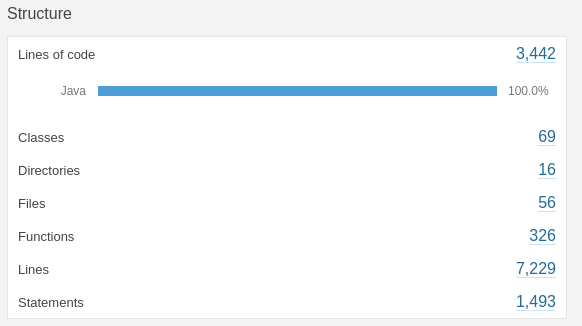
\includegraphics[scale=0.5]{Images/sonarFinal1.png} 
	\caption{Caractéristique de la structure}
	\label{sonarFinal1}
\end{figure} 

\begin{figure}[!h]
	\centering
	\includegraphics[scale=0.5]{Images/sonarFinale2.png} 
	\caption{Caractéristique de la complexité}
	\label{sonarFinal2}
\end{figure} 

\begin{figure}[!h]
	\centering
	\includegraphics[scale=0.5]{Images/sonarFinale3.png} 
	\caption{Pourcentages des commentaires et de la documentation}
	\label{sonarFinal3}
\end{figure} 

\begin{figure}[!h]
	\centering
	\includegraphics[scale=0.5]{Images/sonarFinale4.png} 
	\caption{Répartition des lignes de codes}
	\label{sonarFinal4}
\end{figure} 


\newpage

Le logiciel \textit{SonarQube} peut également effectuer une comparaison globale des deux versions dont on a reporté les résultats dans la figure~\ref{sonarComparaison}. Cette comparaison est très utile car elle permet de mettre en évidence la relation directe des résultats obtenus pour les métriques des deux versions.

\begin{figure}[!h]
	\centering
	\includegraphics[scale=0.5]{Images/sonarcompar.png} 
	\caption{Comparaison globale entre la version initiale et la version finale}
	\label{sonarComparaison}
\end{figure} 

On constate, assez facilement, que les résultats obtenus lors de cette analyse sont similaires aux résultats précédents.

\newpage





\subsubsection{Code dupliqué}
Puisque nous utilisons tous les trois IntelliJ IDEA, l'outil intégré a été utilisé dans un premier temps. La figure \ref{duplicate} montre les résultats obtenus via cette analyse.
On peut noter que les détections ayant un \og coût \fg \, inférieur à $\sim$20 ne sont pas réellement préoccupantes. Pour exemple, les lignes suivantes, extraites de \textit{SquareCoordinateTest}, sont considérées comme dupliquées par l'outil avec un score de 10 :

\begin{java}
assertEquals(square.getSquareAt(Direction.WEST).getY(), 15);
assertEquals(square.getSquareAt(Direction.EAST).getY(), 15);
\end{java}

Il s'agit en effet de 2 lignes très similaires mais il ne nous a pas semblé intéressant de supprimer ce type de duplicat. 
Les parties de code identifiées comme \og duplicats \fg \, et qui nous ont semblé nécessiter un refactoring en ont fait l'objet.

Dans un second temps, nous avons analysé le code via \textit{CPD} inclus dans \textit{PMD} et qui était utilisé dans la suite de rapports à générer par \textit{Maven}. Le seul dupliqué signalé par cet outil concernait la classe \textit{AStarPathTest} pour laquelle les méthodes \textit{hTest} et \textit{gTest} contenaient, en effet, toutes deux ce bloc de code :

\begin{java}
final AStarPath aStarPath = new AStarPath(game);

assertNotNull(aStarPath);
final Player player = game.getPlayers().get(0);
final Square square = player.getSquare();

assertNotNull(player);
assertNotNull(square);

final Square origin = player.getSquare();
final Square destination = player.getSquare().getSquareAt(Direction.EAST);
final Square destination2 = player.getSquare().getSquareAt(Direction.EAST).getSquareAt(Direction.EAST);

final Square destination3 = player.getSquare().getSquareAt(Direction.WEST);
final Square destination4 = player.getSquare().getSquareAt(Direction.WEST).getSquareAt(Direction.WEST);
\end{java}

Ce problème de duplication de code a été résolu en regroupant le contenu des méthodes \textit{hTest} et \textit{gTest} au sein d'une unique méthode de test. En effet, ces deux méthodes ayant un comportement très proche l'un de l'autre, il est évident qu'on puisse les regrouper ensemble.


\begin{figure}[h]
	\centering
	\includegraphics{Images/duplicate_analysis.JPG}
	\caption{\label{duplicate} Recherche de code dupliqué via l'outil intégré à \textit{IntelliJ IDEA}}
\end{figure}

\subsubsection{Audit de code}
\subsubsection*{1) CheckStyle}

\textit{CheckStyle} est un outil de contrôle de code permettant de vérifier le style d'un code source écrit en langage Java.

Egalement intégré dans la suite d'analyses à effectuer via \textit{Maven}, \textit{CheckStyle} a été utilisé avec le \og ruleset \fg \, présent dans la version du code d'origine.
Aucune erreur n'a été détectée mais de nombreux \og warnings \fg \, sont cependant présents (plus de 500). 


La liste suivante présente ces warnings par ordre de nombre de \og violations \fg :\\
\begin{itemize}
	\item 148 violations de type \textit{JavadocStyle} : en réalité toutes des \og First sentence should end with a period. \fg $\rightarrow$ \, la totalité de ces warnings ont été réglés. 
	\item 110 violations de type \textit{MagicNumber} $\rightarrow$ constantes extraites là où cela avait du sens, sauf pour les tests où un tel refactoring nous semblait inutile, nous avons donc supprimé les \og warnings \fg \, pour ceux-ci.
	\item 104 violations de type \textit{LineLength} $\rightarrow$ retours à la ligne là où c'était nécessaire.
	\item 63 violations de type \textit{NeedBraces} $\rightarrow$ bien que nous ne soyons pas tous d'accord sur la valeur ajoutée d'une telle convention, nous avons ajouté les crochets là où \textit{CheckStyle} le demandait.
	\item 35 violations de type \textit{AvoidStarImport} $\rightarrow$ encore une fois désactivés car nous utilisons la fonction \og optimize imports \fg \, d'\textit{IntelliJ IDEA} qui regroupe parfois des imports en un unique via cette notation.
	\item Des violations relatives à des éléments de javadoc manquants $\rightarrow$ Ces éléments ont été ajoutés.
	\item Des violations relatives à des tableaux déclarés à la \og mode C \fg \, plutôt qu' à la \og mode Java \fg $\rightarrow$ \, Des modifications ont été effectuées.
	\item D'autres violations plus \og isolées \fg \, non reprises ici.
\end{itemize}
Comme mentionné ci-dessus, les problèmes de style ont été réglés et on a retrouve donc bien la situation du code d'origine : aucun avertissement pour de tels problèmes.

\subsubsection*{2) IntelliJ Code inspection}

C'est un outil d'analyse de code qui applique des inspections sur celui-ci. Il permet de détecter les erreurs de compilations mais aussi les différentes inefficacité présents dans le code.

\paragraph{Détection d'une partie de condition impliquant QUICK\_WIN comme \og pointless \fg : } 
Puisque la variable \textbf{QUICK\_WIN} est mise à \og true \fg \, ou \og false \fg \, dans le code et pas par un paramètre pouvant varier au runtime, la version compilée contient effectivement une (partie de ) condition qui n'a pas vraiment de sens (toujours vraie ou fausse).
Néanmoins, bien qu'il eut été possible de faire varier sa valeur \og dynamiquement \fg \, (par un paramètre optionnel au lancement du programme par exemple), nous n'avons pas jugé utile d'implémenter une telle fonctionnalité. En effet, il s'agit surtout d'une option de développement permettant de tester une suite de niveau, pas d'une \og feature \fg \, destinée aux utilisateurs (sa présence dans le code au stade de la release ayant pour but de faciliter le travail des \og évaluateurs \fg).
\paragraph{Altérations mineures diverses}

\begin{itemize}
	\item La variable de classe \og Level \fg{} dans \mbox{\textit{SinglePlayerTest}} fut convertie en variable locale,
	\item 4 booléens n'avaient aucun intérêt et furent donc ôtés,
	\item 6 paramètres avaient toujours la même valeur et furent donc remplaçés par celle-ci,
	\item 2 paramètres n'étaient jamais utilisés et furent ôtés,
	\item 14 accès furent rendus plus restrictifs,
	\item La valeur de retour de la méthode \mbox{\textit{Level/PlayerMoveTask\#run()}} n'était pas utilisée et cette méthode a donc été convertie en \og void \fg{},
	\item 8 variables ont été déclarées \og final \fg{},
	\item 11 éléments étaient reportés inutilisés, ceux qui n'avaient pas d'usage ont été enlevés (les autres sont suite à la gestion du score de fonctionnalités non implémentées),
	\item Les 5 constantes dans \mbox{\textit{SinglePlayerTest\#constantTest()}} étaient accédées par référence d' instance, elles sont maintenant accédées par référence de classe. De même dans \mbox{\textit{AStarPathTest}},
	\item 7 types anonymes ont été remplaçés par des expressions lambda,
	\item 3 déclarations de type explicites furent remplaçés par \og <> \fg{} dans le contexte de listes,
	\item 2 boucles de type \og for each \fg{} furent remplaçées par des flux,
	\item Intellij a soulévé 3 erreurs dans la Javadoc, qui furent corrigées,
	\item 6 \og asserts \fg{} étaient toujours vrais, ils ne le sont plus.
\end{itemize}
\paragraph{\og Warnings \fg \ sur des \og problèmes de modernité \fg : }
Ces signalements, surtout liés au code dans sa version de base (avant nos changements individuels), se présentaient par exemple aux endroits où un \og for indexé \fg \, pouvait être remplacé par un \og foreach \fg \, ou bien lorsqu'une classe anonyme \og classique \fg \, pouvait disparaitre au profit d'une expression lambda. Les \og modernisations \fg \, ont donc été effectuées (pour la plupart grâce à des \og refactorings \fg \, automatiques d'\textit{IntelliJ IDEA}).

\paragraph{Classe obsolète : }
La classe \mbox{\textit{DefaultPlayerInteraction}} était non utilisée et, comme nous avons modifié les interactions lors de collisions, elle n'avait pas été mise à jour.
Elle a donc été supprimée.

\subsubsection*{3) PMD}

\textit{PMD} est un framework qui permet d'analyser le code source Java. Il contient un certain nombre de règles qui assurent la qualité du code : le code inutile, les imbrications trop complexes,... Il permet d'obtenir les résultats par le biais d'un rapport.

\paragraph{\og Feature envy \fg \, potentiel lié à la récupération des cases \og safe \fg : }
Lorsque le joueur doit être téléporté vers une case à l'écart des fantômes, il est nécessaire de regarder le contenu du \textit{Board}. Il est donc logique que ce soit celui-ci qui se charge de récupérer la liste des cases \og safe \fg . De fait, pour éviter un problème potentiel de \og feature envy \fg , cette récupération a été déplacée de \textit{Level} vers \textit{Board}.
\paragraph{Détection de \og God classes \fg : }
Signifie en principe que :
\begin{enumerate}
	\item la classe a une \og cohésion interne \fg faible
	\item la classe accède à des attributs appartenant à trop de classes étrangères
	\item la classe est trop complexe par rapport à sa taille
\end{enumerate}
En regardant dans le code de PMD \footnote{\url{https://pmd.github.io/pmd-5.4.1/pmd-java/xref/net/sourceforge/pmd/lang/java/rule/design/GodClassRule.html}}, il semblerait que la valeur de complexité (cyclomatique apparemment) de la classe soit bien calculée mais qu'à aucun moment une pondération par rapport à la taille de celle-ci (nombre de méthodes par exemple) ne soit faite, ce qui ne respecte pas la définition d'origine.
Les classes qui contiennent beaucoup de méthodes sont donc naturellement sujettes à un signalement de type \og god class \fg.

Bien que, comme expliqué ci-dessus, la détection ne soit pas parfaite, nous avons choisi de réagir pour éviter qu'une classe n'aie trop de méthodes. Les changements effectués ont effectivement permis de supprimer les avertissements en question tout en permettant probablement à notre code d'être plus \og maintenable \fg \, puisque les classes sont globalement moins volumineuses.

La classe \mbox{\textit{Player}} regroupait l'implémentation de deux fonctionnalités séparées (score et labyrinthe) en plus des services de base, dès lors, il a été préféré de la diviser en plusieurs: le comportement lié à la fonctionnalité \og score \fg a été déplaçé dans la classe descendante \mbox{\textit{IdentifiedPlayer}} et les méthodes de vérification de contenu de fichiers ont été déplaçées vers \mbox{\textit{FileChecker}}.
A ce jour, il ne reste plus de \og god class \fg dans l'implémentation.


\paragraph{Taille de code : }

Deux classes (\mbox{\textit{Player}} et \mbox{\textit{Launcher}}) avaient trop de méthodes, donc certaines furent déplaçées ou intégrées à une méthode appelante lorsque c'était possible.

La méthode \mbox{\textit{PacManhattanAI\#BFSNearestPelletSquare()}}) avaient une complexité cyclomatique trop élevée, elles ont donc été l'object de \og refactorings \fg afin de réduire celle-ci.

\paragraph{Loi de Demeter : }

PMD détecte de nombreuses violations par rapport à cette loi, mais beaucoup d'entre elles viennent du code originel et la vaste majorité relèvent d'appels à des librairies standard Java, il nous a donc paru que la détection de PMD était inadéquate à ce niveau.
Pour ce qui est des autres violations, le code existant force largement à les commettre.

\paragraph{Avertissements mineurs}

\begin{itemize}
	\item Deux \og if \fg{} imbriqués dans \mbox{\textit{PlayerMoveTask\#run()}} furent intégrés en un seul,
	\item 9 Arraylists furent convertis en List et une Hasmap en Map,
	\item 4 \og varargs \fg{} furent introduits là où c'était possible,
	\item 5 déclarations d'attributs de classe furent déplaçés à la tête de leur classe,
	\item 15 \og assert \fg{} furent modifiés pour éviter la surdépendance à \og assertTrue() \fg{},
	\item 251 messages d'erreur furent ajoutés aux \og assert \fg{} qui en étaient privés,
	\item Certaines variables au nom trop court furent renommées, d' autres non (variable à l'étendue fort restreinte ou correspondant à des coordonnées cartésiennes),
	\item Des méthodes, variables, classes et constantes ont été renommées pour correspondre aux conventions du langage,
	\item De nombreuses variables et paramètres furent déclarés \og final \fg{},
	\item L'initialisation superflue de \mbox{\textit{PlayerMoveTask\#finished}} a été ôtée.
\end{itemize}

\subsubsection*{4) FindBugs}

\textit{FindBugs} est un logiciel libre d'analyse statique de bytecode Java. Il a pour objectif de trouver des bugs dans les programmes Java en identifiant des patterns reconnus comme étant des bugs.

Cet outil a détecté que plusieurs opérations d' écriture et lecture de fichiers ne spécifiaient pas le \og charset \fg utilisé et que certaines opérations de concaténation de chaînes de caractères étaient effectuées dans des boucles.
les opérations de lecture et d' écriture de fichier spécifient maintenant le \og charset \fg et les concaténations de chaînes de caractères ont été remplacées par des \og StringBuilder.append() \fg.
\subsection{Analyse dynamique}

Nous allons maintenant exécuter le code et observer le comportement du logiciel dans ce cas. Nous allons également évaluer la portée des tests unitaires afin de vérifier que tout le code (ou une bonne partie) est couverte et donc testées.

\subsubsection{Couverture du code}

La couverture du code est importante pour connaître les portions de code inutiles, non testées, ou jamais appelées à l'exécution du logiciel.

\paragraph{Couverture globale}

Avant l'ajout de nos fonctionnalités, le pourcentage de code couvert par des tests était comme suit: 

\begin{figure}[!h]
	\centering
	\includegraphics[width=\textwidth]{Images/InitialCoverage}
	\caption{\label{InitialCoverage} Rapport de couverture de code généré par \textit{IntelliJ IDEA} sur le code initial}
\end{figure}


Actuellement, ces pourcentages ont évolué de la manière suivante:

\begin{figure}[!h]
	\centering
	\includegraphics[width=\textwidth]{Images/MergedCoverage}
	\caption{\label{MergedCoverage} Rapport de couverture de code généré par \textit{IntelliJ IDEA} sur notre code}
\end{figure}

\newpage
Comme on peut le voir, la couverture globale a non seulement été maintenue dans l'ensemble, mais a augmenté légèrement à tous les niveaux.

\paragraph{Classes où la couverture de code a diminué significativement : }

\begin{itemize}
	\item La classe \mbox{\textit{BoardFactory}} a vu sa couverture diminuer de 6,7\% au niveau des méthodes et 27,2\% au niveau des lignes étant donné que certaines méthodes liées à la conversion d'images en fichiers de niveaux ne sont pas testées (la conversion en elle-même est testée mais les méthodes l'appelant non, car trop dépendantes des fichiers présents, qui peuvent varier).
	\item La classe \mbox{\textit{PlayerCollisions}} a subi une légère baisse de sa couverture de lignes de 6,7\% du fait qu' une clause \og catch \fg ne soit évidemment pas testée.
\end{itemize}

Dans le cas des classes préexistantes non mentionnées ci-haut, la couverture s'est soit maintenue, soit a été accrue, parfois fortement.

\paragraph{Classes et packages ajoutés : }

\begin{itemize}
	\item La classe \mbox{\textit{MyJDialogStrategy}} a une couverture de 100\% au niveau des classes, 71,4\% au niveau des méthodes et 69;8\% au niveau des lignes. Les méthodes et lignes non testées dépendent d'une action du joueur.
	\item La classe \mbox{\textit{IdentifiedPlayer}} est couverte à hauteur de 100\% au niveau des classes, 85,7\% au niveau des méthodes et 65,6\% au niveau des lignes. Les méthodes et lignes non testées sont liées à des affichages graphiques.
	\item La classe \mbox{\textit{AILevel}} jouit d' une couverture de 66,7\% au niveau des classes, 61,5\% au niveau des méthodes et 64,4\% au niveau des lignes. Les méthodes et lignes non testées dépendent d'un jeu en exécution.
	\item La classe \mbox{\textit{HallOfFame}} bénéficie d'une couverture de 100\% au niveau des classes, 91,7\% au niveau des méthodes et 72,7\% au niveau des lignes. Les méthodes et lignes non testées sont liées à des affichages graphiques et gestions d' exceptions.
	\item L' énumération \mbox{\textit{Achievement}} se voit testée pour 100\% au niveau des classes, 100\% au niveau des méthodes et 92,9\% au niveau des lignes. Les lignes non testées correspondent à une gestion d' exceptions.
	\item L' énumération \mbox{\textit{ItemsColor}} est entièrement couverte.
	\item La classe utilitaire \mbox{\textit{FileChecker}} dispose d'une couverture de code de 100\% au niveau des classes, 66,7\% au niveau des méthodes et 51,2\% au niveau des lignes. Le contenu non couvert correspond essentiellement à une méthode de lecture de fichier, en corrélation avec la nature de la classe.
	\item Le package \mbox{\textit{Strategy}} est couvert pour 100\% au niveau des classes, 95,9\% au niveau des méthodes et 88,8\% au niveau des lignes.\\ 
	
Les classes ci-dessous appartiennent à ce package :\\ 
	\item Les classes \mbox{\textit{AIStrategy}} et \mbox{\textit{HumanControllerStrategy}} sont entièrement couvertes.
	\item La classe \mbox{\textit{AStar}} a une couverture de 100\% au niveau des classes, 100\% au niveau des méthodes et 96,4\% au niveau des lignes.
	\item La classe \mbox{\textit{AStarPath}} a une couverture de 100\% au niveau des classes, 100\% au niveau des méthodes et 90,6\% au niveau des lignes.
	\item La classe \mbox{\textit{PacmanStrategy}} a une couverture de 100\% au niveau des classes, 100\% au niveau des méthodes et 90,9\% au niveau des lignes.
	\item La classe \mbox{\textit{PacManhattanAI}} a une couverture de 100\% au niveau des classes, 92,9\% au niveau des méthodes et 81,7\% au niveau des lignes. Les méthodes et lignes non testées dépendant de la classe \textit{AStar} qui n'a pas semblé utile de tester car c'est une classe template (voir section \ref{IA}).
\end{itemize}


\paragraph{Mesures prises pour améliorer la couverture de code : }
L'analyse de couverture du code a révélé trois problèmes.

\begin{enumerate}
\item En premier lieu, nous avions \og court-circuité \fg les tests de l'interface graphique du jeu en lui-même, ceux-ci ont donc été réinstaurés.

\item En deuxième lieu, une méthode (\mbox{\textit{Achievement\#offerAchievements()}}) ajoutée tardivement n'était pas testée, le test a donc été rajouté.

\item Enfin, des tests furent rajoutés pour la classe \mbox{\textit{PacManhattanAI}}.
\end{enumerate}



\subsubsection{Profilage}

Le profilage permet de connaître les parties de codes qui peuvent être problématiques en terme de performances. Les méthodes mises en évidence peuvent être mal optimisée et donc ralentir le logiciel de manière importante.


Pour cette partie de l'analyse dynamique, il sera fait usage de \textit{Yourkit} (version d'évaluation complète). \textit{Yourkit} est un profiler pour les applications écrites en Java créé par la société Yourkit LLC en 2003.  On tente ici de déterminer si des endroits du code monopolisent les ressources CPU/RAM et, le cas échéant, lesquels.\\


On réalisera 2 scénarios :
\begin{itemize}
	\item Jeu en mode "IA" qu'on laisse tourner jusqu'à la mort définitive de Pac-man
	\item Jeu en mode "Joueur" pour lequel on crée un compte, on s'y connecte et, lorsque Pac-man perd sa dernière vie, on recommence une fois la partie en chargeant le niveau 1
\end{itemize}
\paragraph{Processeur et threads : }
Pour les deux scénarios susmentionnés, l'analyse montre que la méthode \mbox{\textit{Navigation\#shortestPath(Square, Square, Unit)}} et en particulier l'appel à \mbox{\textit{HashSet.add(Object)}} prend l'écrasante majorité du temps CPU. La figure \ref{hotspot} montre le résultat de l'analyse \og Hot spots \fg \, de \textit{Yourkit} sur le scénario "Joueur" (les résultats sur l'autre scénario étant similaires).
\begin{figure}[h]
	\centering
	\includegraphics[width=16cm]{Images/hotspot.JPG}
	\caption{\label{hotspot} Recherche d' \og Hot spots \fg \, CPU avec \textit{Yourkit}}
\end{figure}

On constate donc que l'intelligence artificielle des fantômes (qui était présente dans la version originale du jeu) est gourmande en ressources par rapport au reste du programme, il serait donc intéressant de s'assurer que son comportement est optimisé. Cependant, il nous semble l'être et il n'est pas étonnant que le comportement d'intelligences artificielles prenne du temps CPU. On note également que des méthodes liées à l'affichage et à la gestion des entrées/sorties sont détectées comme \og Hot spots \fg \, bien que leur impact soit négligeable en comparaison.

De manière générale, on peut voir l'évolution au cours du temps de l'utilisation du processeur et du nombre de threads sur les graphes de la figure \ref{cpu-threads}. Toujours rien d'anormal à ce stade.
\begin{figure}[h]
	\centering
	\includegraphics{Images/cpu-threads.JPG}
	\caption{\label{cpu-threads} Evolution de l'utilisation CPU et du nombre de threads avec \textit{Yourkit}}
\end{figure}
\paragraph{Mémoire : }
Pour les deux scénarios considérés, on constate que la mémoire utilisée reste assez constante, tout comme le nombre de passages du \og Garbage Collector \fg. La figure \ref{memory} rend compte des principaux résultats obtenus pour le scénario "IA".
\begin{figure}[h]
	\centering
	\includegraphics[width=16cm]{Images/memory.JPG}
	\caption{\label{memory} Utilisation mémoire avec \textit{Yourkit}}
\end{figure}

On ne constate donc toujours pas de problème pour cette partie ci de l'analyse. On notera, comme le montre l'image, qu'il a été choisi de ne montrer que la mémoire utilisée en terme de \og metaspace \fg \, pour la mémoire \og non-heap \fg. Cela vient du fait que \textit{Yourkit} analyse également le \og Code Cache \fg, qui augmente continuellement (comportement de Java qui garde en cache du code) et donne donc une fausse impression d'augmentation.

Il ne nous a pas semblé intéressant de \og profiler \fg \, la version de JPacman originelle puisque nous n'avons pas repéré de problèmes à ce stade ci alors que la version finale comprend une IA pour Pac-man, nécessitant donc naturellement plus de ressources (pour le moins en termes de CPU).

\subsection{Interprétation de la qualité}

Après avoir effectué cette analyse de qualité et la comparaison de celle-ci entre la version initiale et la version finale de JPacman, on peut en conclure que la qualité du code source après intégration (version finale) est tout à fait convenable par rapport aux modifications qui ont été effectuées sur le version initiale. En effet, que ce soit au niveau des métriques, du code dupliqué, de la couverture de code,... ou encore du profilage, on peut constater que les résultats obtenus lors des analyses sont tout à fait acceptables et sont parfois très semblables aux résultats de la version initiale grâce à d'importantes améliorations de la qualité qui ont été effectuées pour obtenir la version finale.


\section{Analyse de l'évolution du logiciel}

Dans cette section, une analyse de l'évolution du logiciel en terme de nombre de lignes de code est effectuée. Pour cela, l'outil \textit{SLOCCount}\footnote{http://www.dwheeler.com/sloccount/} a été utilisé. Cet outil permet une première analyse très sommaire du code source d'un projet. En effet, il permet de compter les lignes de code que contiennent les fichiers de code source. Il permet donc d'analyser l'évolution du nombre de lignes de code en fonction du temps pour vérifier que celle-ci ne prenne pas de l'ampleur trop rapidement.

Nous allons appliquer cet outil sur trois versions et discuter des résultats qu'il fournit. Les trois versions qui seront analysées sont les suivantes : 

\begin{enumerate}
\item La version initiale
\item la version juste après intégration des trois fonctionnalités
\item la version finale (après refactorings)
\end{enumerate}

Les résultats retournés sont reportés en graphique dans la figure~\ref{evolution}.

\begin{figure}[h]
	\centering
	\includegraphics[scale=0.5]{Images/evolution.png} 
	\caption{\label{evolution} Nombre de lignes de code calculés pour chaque version avec \textit{SLOCCount}}
\end{figure}

Au vu de ces résultats, nous pouvons constater qu'au fil des versions, le projet prend de l'ampleur. Ce qui est évidemment logique vu qu'au fil du temps, des fonctionnalités ont été ajoutées au logiciel initial. Ensuite, nous constatons qu'il y a une diminution du nombre de lignes de codes. Ce comportement de la courbe, peut être facilement expliqué par la phase de \textit{refactoring} qui a succédé à l'intégration des fonctionnalités individuelles. On constate que cette phase a eut un impact positif sur le nombre de lignes de code car elle a permis de diminuer ce chiffre.

\newpage
\section{Notes diverses et guide d'utilisation}
\subsection{Maven}
Le projet utilisant Maven\footnote{\url{https://maven.apache.org/}}, il est très facile de compiler le code, de l'analyser avec les outils prévus ou d'exécuter la suite de tests.
On peut noter que la configuration originale du projet ne permettait pas l'exécution de l'archive jar produite, cela a été corrigé pour notre version (en reproduisant simplement les dépendances externes dans l'archive générée, via un plugin).

En considérant que Maven est correctement installé sur votre machine et en plaçant un terminal (une invite de commande ou autre terme décrivant une \og console \fg \, sur votre système d'exploitation) à la racine du projet (c'est-à-dire l'endroit où se trouve le fichier \nolinkurl{pom.xml}), vous pouvez :
\begin{itemize}
	\item Exécuter les tests via :
	\begin{lstlisting}[language=bash]
	$ mvn test
	\end{lstlisting}
	\item Compiler le projet (inclus l'exécution des tests) via :
	\begin{lstlisting}[language=bash]
	$ mvn compile
	\end{lstlisting}
	\item Lancer le jeu via (après avoir compilé) via :
	\begin{lstlisting}[language=bash]
	$ mvn exec:java -Dexec.mainClass=
		"nl.tudelft.jpacman.Launcher"
	\end{lstlisting}
	\item Compiler le projet et produire une archive "jar" exécutable via :
	\begin{lstlisting}[language=bash]
	$ mvn package
	\end{lstlisting}
	L'archive est ensuite exécutable via :
	\begin{lstlisting}[language=bash]
	$ java -jar target/jpacman-framework-7.3.0.jar
	\end{lstlisting}
	\item Générer le site Maven (inclus les étapes précédentes, la javadoc et des rapports d'analyse) via :
	\begin{lstlisting}[language=bash]
	$ mvn site
	\end{lstlisting}
	(le site généré étant accessible en ouvrant \nolinkurl{target/site/index.html})
	\item D'autres commandes sont évidemment disponibles pour, par exemple, générer la javadoc séparément mais ne sont pas reprises ici.
\end{itemize}

\subsection{Travis}
Puisque le projet JPacman dans son état \og initial \fg \, (avant modifications de notre part) intégrait déjà le fichier de configuration Travis\footnote{\url{https://travis-ci.org/}}, nous l'avons utilisé sur nos différents \og forks \fg .

Les historiques des \og builds \fg \, (avec leurs logs) de la version d'intégration et de la version individuelle d'Adrien Coppens sont disponibles à l'adresse : \url{https://travis-ci.org/qdrien/jpacman-framework/builds}.

L' historique des \og builds \fg \, (avec leurs logs) de la version individuelle de Nicolas Leemans est disponible à l'adresse : \url{https://travis-ci.org/NicolasLeemans7/jpacman-framework/builds}.

\subsection{Organisation des dépots Git(Hub)}
Les versions correspondant à la phase individuelle sont disponibles aux adresses suivantes :
\begin{itemize}
	\item Adrien Coppens (extension \og Série de labyrinthes \fg ) : 
	
	\url{https://github.com/qdrien/jpacman-framework}
	
	Tag de la release : \nolinkurl{individual-coppens-series-of-mazes-v7.0.0}
	
	(sur la branche \nolinkurl{series-of-maze})
	\item Damien Legay (extension \og Score \fg ) : 
	
	\url{https://github.com/DamienLegay/jpacman-framework}
	
	Tag de la release : \nolinkurl{}{Final\_Release}
	\item Nicolas Leemans (extension \og IA pour Pacman \fg ) : 
	
	\url{https://github.com/NicolasLeemans7/jpacman-framework}
	
	Tag de la release : \nolinkurl{individual-leemans-AI-for-Pacman-v7.0.0}
	(sur la branche \nolinkurl{Master})
\end{itemize}

Le dépot commun pour la phase d'intégration est celui d'Adrien Coppens, la release finale étant taggée \nolinkurl{}. %todo

%todo: build la javadoc et l'ajouter au repo!!!
%todo: optimize imports/reformat code!!!
%todo: + tagger la release finale


\subsection{Spécificités des ajouts individuels}
\subsubsection{Fonctionnalité "Série de labyrinthes"}
\begin{itemize}
	\item Afin de pouvoir tester différents niveaux plus aisément, un booléen \mbox{\textbf{QUICK\_WIN}} est configurable dans la classe \mbox{\textit{Level}}.
	Si on lui affecte la valeur \textit{true}, récupérer treize gommes est suffisant pour réussir un niveau (et passer au suivant).
	\item Les fichiers correspondants aux niveaux disponibles en jeu se trouvent dans le répertoire \nolinkurl{target/classes} à condition d'avoir au moins \og compilé \fg la solution via la commande :
	\begin{lstlisting}[language=bash]
	$ mvn compile
	\end{lstlisting}
	(Toute commande permettant l'exécution d'une étape postérieure du cycle Maven\footnote{\url{https://maven.apache.org/guides/introduction/introduction-to-the-lifecycle.html}} est également recevable)
	
	Avant compilation, ces mêmes fichiers se trouvent dans \nolinkurl{src/main/resources}.
	\item Un niveau numéroté $n$ est considéré comme partie intégrante du jeu si le fichier "\nolinkurl{board}$n$\nolinkurl{.txt}" est présent et si les fichiers des niveaux $1...n-1$ le sont également.
	\item Au lancement du jeu, si le fichier "\nolinkurl{board}$n$\nolinkurl{.txt}" est manquant mais qu'il existe un fichier "$n$\nolinkurl{.png}", le \og convertisseur de carte \fg \,  mentionné au paragraphe ad hoc de la section \ref{map_generator_txt} en page \pageref{map_generator_txt} crée le fichier "\nolinkurl{board}$n$\nolinkurl{.txt}" correspondant.
\end{itemize}

\section{Conclusion}

Ce projet nous a permis de mettre en pratique les différents concepts vu au cours de Software Evolution, notamment en matière de qualité d'un logiciel, maintenabilité du code, mise en place d'évolution du logiciel ainsi que la surveillance de l'évolution du code. Le projet nous a également permis de nous familiariser avec différents outils de gestion d'un code source, d'analyse et de refactoring. Ces outils nous ont permis d'identifier des problèmes fréquents et potentiels dans le code source, qui peuvent altérer la qualité et rendre l'évolution d'un système plus complexe.

JPacman était un projet relativement bien conçu à la base mais il y avait notamment des petits problèmes de qualité. Nous nous sommes rendus compte également qu'il fallait rester vigilant concernant les résultats fournis par des outils logiciels car ceux-ci peuvent parfois provoquer des problèmes, par exemple du code dupliqué qui ne l'est pas vraiment ou des avertissements que l'on peut considérer comme sans gravité. De plus, les tests unitaires ont permis de gérer les évolutions et les erreurs commises en gardant un contrôle tout au long du processus de développement en effectuant des tests de régression et de validation.

En ce qui concerne la version finale du logiciel, celle-ci a une qualité globalement satisfaisante selon les critères analysées. En effet, par rapport aux modifications qui ont été effectuées lors des extensions, nous sommes parvenus à conserver une complexité plutôt correcte par rapport à la difficulté des fonctions ajoutées telle que l'IA. Ce projet nous a montré que l'ajout de fonctionnalité supplémentaires rend particulièrement difficile la conservation d'une complexité raisonnable si l'on ne tient pas compte des critères d'évaluations de qualité.


\end{document}
